\documentclass[10pt,twocolumn,letterpaper]{article}
\usepackage[10pt,inchmargins]{sigmin}  %% template from Xi Wang.
\special{papersize=8.5in,11in}
\setlength{\pdfpagewidth}{8.5in}
\setlength{\pdfpageheight}{11in}
\usepackage[noheadfoot,
            left=1in,right=1in,top=1in,bottom=1in,
            columnsep=0.3in
            ]{geometry}
\usepackage[small,compact]{titlesec}
\usepackage[font={small,bf}]{caption}    % added 9/10/13
\usepackage[nolineno,noindent,norules]{lgrind}
\usepackage{tightenum}
\usepackage{float}
\usepackage{xspace}
\usepackage{times,pifont}
\usepackage{mathptmx}
\usepackage{subfig,graphics,graphicx,color}
\usepackage{multirow}
\usepackage{dblfloatfix} %% correctly orders single- and double-col figures
\usepackage{hyphenat}
\usepackage{mathrsfs}
\usepackage{subfig}
\usepackage{amssymb,amsmath,centernot}
\usepackage{lastpage}
\usepackage{flushend}
\usepackage{hhline}
\usepackage{authblk}
\newcommand{\doi}{10.1145/2517349.2522735}


%%% ================= START of SOSP '13 template ================= 
\makeatletter

\def\ftype@copyrightbox{8}
\def\@copyrightspace{
\@float{copyrightbox}[b]
\begin{center}
\setlength{\unitlength}{1pc}
\begin{picture}(20,6.0) 
\put(0,3){\parbox{\columnwidth}{\scriptsize

%*** SAMPLE. AUTHOR PUT SUPPLIED TEXT HERE ****

\noindent
\rule{6.0 cm}{0.2pt}\\
Permission to make digital or hard copies of part or all of this work 
for personal or classroom use is granted without fee provided that
copies are not made or distributed for profit or commercial advantage 
and that copies bear this notice and the full citation on the first
page. Copyrights for third-party components of this work must be
honored.  For all other uses, contact the Owner/Author. 

\vspace{\baselineskip}\noindent
Copyright is held by the Owner/Author(s).\\
\textit{SOSP'13}, Nov. 3--6, 2013, Farmington, Pennsylvania, USA. \\
ACM 978-1-4503-2388-8/13/11.

\noindent
http://dx.doi.org/\doi}
}
\end{picture}
\end{center}
\end@float}

\def\maketitle{\par
 \begingroup
   \def\thefootnote{\fnsymbol{footnote}}
   \def\@makefnmark{\hbox
       to 0pt{$^{\@thefnmark}$\hss}}
     \twocolumn[\@maketitle]
\@thanks
 \endgroup
 \setcounter{footnote}{0}
 \let\maketitle\relax
 \let\@maketitle\relax
 \gdef\@thanks{}\gdef\@author{}\gdef\@title{}\gdef\@subtitle{}\let\thanks\relax
 \@copyrightspace}

\makeatother

%%% ================= END of SOSP '13 template ================= 



\newcommand{\comment}[1]{}
\frenchspacing

%\doublespacing

%%%%%%%%%%%%%%%%%%%%%%%%%%%%
%     macro

\newcommand{\xxx}{\mbox{\textsc{Parrot}}\xspace}
\newcommand{\mytitle}[0]{\textbf {\xxx: A Practical Runtime \\
  for Deterministic, Stable, and Reliable Threads}}
\newcommand{\mykeywords}[0]{Deterministic Multithreading, Stable Multithreading,
  Software Model Checking, State Space Reduction}

%%%%%%%%%%%%%%%%%%%%%%%%%%%%%%%%%%%%%%%%%%%%%%%%%%%%%%%%%%%%%%%%%
% hyperref stuff

\usepackage[square,comma,numbers,sort]{natbib}
\usepackage{hypernat}
\usepackage{hyperref}

%% fill in pdf info here
\hypersetup{%
colorlinks=false,
pdfborder={0 0 0},
pdftitle={\mytitle},
pdfkeywords={\mykeywords},
bookmarksnumbered,
pdfstartview={FitH},
urlcolor=cyan,
pdfpagelabels=true,
pdfdisplaydoctitle=true,
}%

%\usepackage{breakurl}
%\usepackage[all]{hypcap}
%\renewcommand{\url}{\burl}

%%%%%%%%%%%%%%%%%%%%%%%%%%%%%%%%%%%%%%%%%%%%%%%%%%%%%%%%%%%%
% Some NICE fonts

\newfont{\BIG}{cminch}                             %--- One-inch font
\newfont{\sfbHuge}{cmssbx10 scaled\magstep5}       %-- 25pt sans serif bold
\newfont{\sfbLarger}{cmssbx10 scaled\magstep3}   %-- 12+pt sans serif boldd
\newfont{\sfblarger}{cmssbx10 scaled\magstep2}   %-- 12+pt sans serif bold
\newfont{\sfblarge}{cmssbx10 scaled\magstep1}      %-- 12pt sans serif bold
\newfont{\sfbeleven}{cmssbx10 scaled\magstephalf}  %-- 11pt sans serif bold
\newfont{\sfb}{cmssbx10}                           %-- 10pt sans serif bold
\newfont{\sfeight}{cmss8}                          %-- 8pt sans serif

%%%%%%%%%%%%%%%%%%%%%%%%
%    space tweaking

%\textwidth = 6.5 in
%\textheight = 9.0 in
%\setlength{\topmargin}{-.5in}

%\headheight = 0.0 in
%\headsep = 0.0 in
%\parskip = 0.2in
%\parindent = 0.0in

\renewcommand{\topfraction}{0.95}
\addtolength{\textfloatsep}{-0.1in}
%\addtolength{\floatsep}{0.025in}
\renewcommand\floatpagefraction{.9}
%\renewcommand\bottomfraction{.9}
\renewcommand\textfraction{.1}

\setlength{\parindent}{9pt}

% Rescue
\makeatletter
\def\v#1{{\mbox{\fontfamily{cmtt}\fontsize{\f@size}{\f@size}\selectfont #1}}}
\newcommand{\compute}{soft barrier\xspace}
\newcommand{\vcompute}{\emph{soft barrier}\xspace}
\newcommand{\computes}{soft barriers\xspace}
\newcommand{\Compute}{Soft barrier\xspace}
\newcommand{\Computes}{Soft barriers\xspace}
\newcommand{\nondet}{performance critical section\xspace}
\newcommand{\vnondet}{\emph{performance critical section}\xspace}
\newcommand{\nondets}{performance critical sections\xspace}
\newcommand{\Nondet}{Performance critical section\xspace}
\newcommand{\Nondets}{Performance critical sections\xspace}

\newcommand{\dmt}[0]{DMT\xspace}
\newcommand{\smt}[0]{StableMT\xspace}
\newcommand{\racepro}[0]{\textsc{RacePro}\xspace}
\newcommand{\tern}[0]{\textsc{Tern}\xspace}
\newcommand{\peregrine}[0]{\textsc{Peregrine}\xspace}
\newcommand{\grace}[0]{Grace\xspace}
\newcommand{\coredet}[0]{\textsc{CoreDet}\xspace}
\newcommand{\kendo}[0]{Kendo\xspace}
\newcommand{\dthreads}[0]{\textsc{DThreads}\xspace}
\newcommand{\determinator}[0]{Determinator\xspace}
\newcommand{\dbug}[0]{\textsc{dbug}\xspace}
\newcommand{\ecosys}[0]{\xxx-\dbug}

\newcommand{\apache}{\v{Apache}\xspace}
\newcommand{\ab}{\v{ApacheBench}\xspace}
\newcommand{\mysql}{\v{MySQL}\xspace}
\newcommand{\sysbench}{\v{SysBench}\xspace}
\newcommand{\mplayer}[0]{{MPlayer}\xspace}
\newcommand{\mencoder}[0]{\v{mencoder}\xspace}
\newcommand{\pbzip}[0]{\v{PBZip2}\xspace}
\newcommand{\aget}[0]{\v{aget}\xspace}
\newcommand{\mongoose}[0]{\v{Mongoose}\xspace}
\newcommand{\pfscan}[0]{\v{pfscan}\xspace}
\newcommand{\fft}[0]{\v{fft}\xspace}
\newcommand{\luc}[0]{\v{lu\_cb}\xspace}
\newcommand{\lun}[0]{\v{lu\_ncb}\xspace}
\newcommand{\barnes}[0]{\v{barnes}\xspace}
\newcommand{\radix}[0]{\v{radix}\xspace}
\newcommand{\radiosity}[0]{\v{radiosity}\xspace}
\newcommand{\waters}[0]{\v{water-spatial}\xspace}
\newcommand{\watern}[0]{\v{water-nsquared}\xspace}
\newcommand{\oceanncp}[0]{\v{ocean}\xspace}
\newcommand{\oceancp}[0]{\v{ocean}\xspace}
\newcommand{\fmm}[0]{\v{fmm}\xspace}
\newcommand{\volrend}[0]{\v{volrend}\xspace}
\newcommand{\cholesky}[0]{\v{cholesky}\xspace}
\newcommand{\streamcluster}[0]{\v{streamcluster}\xspace}
\newcommand{\blackscholes}[0]{\v{blackscholes}\xspace}
\newcommand{\swaptions}[0]{\v{swaptions}\xspace}
\newcommand{\bodytrack}[0]{\v{bodytrack}\xspace}
\newcommand{\bodytrackopenmp}[0]{\v{bodytrack-openmp}\xspace}
\newcommand{\ferret}[0]{\v{ferret}\xspace}
\newcommand{\dedup}[0]{\v{dedup}\xspace}
\newcommand{\raytrace}[0]{\v{raytrace}\xspace}
\newcommand{\canneal}[0]{\v{canneal}\xspace}
\newcommand{\racey}[0]{\v{racey}\xspace}
\newcommand{\freqmine}[0]{\v{freqmine}\xspace}
\newcommand{\vips}[0]{\v{vips}\xspace}
\newcommand{\xtwosixfour}[0]{\v{x264}\xspace}
\newcommand{\fluidanimate}[0]{\v{fluidanimate}\xspace}
\newcommand{\facesim}[0]{\v{facesim}\xspace}
\newcommand{\rtviewraytrace}[0]{\v{rtview\_raytrace}\xspace}
\newcommand{\wordcount}[0]{\v{word\_count}\xspace}
\newcommand{\klee}[0]{\textsc{klee}\xspace}
\newcommand{\woodpecker}[0]{\textsc{woodpecker}\xspace}
\newcommand{\splashx}[0]{\mbox{SPLASH-2x}\xspace}
\newcommand{\parsec}[0]{\mbox{PARSEC}\xspace}
\newcommand{\phoenix}[0]{\mbox{Phoenix}\xspace}
\newcommand{\pthread}[0]{\mbox{Pthreads}\xspace}

\newcommand{\kmeans}[0]{\v{kmeans}\xspace}
\newcommand{\kmeanspthread}[0]{\v{kmeans-pthread}\xspace}
\newcommand{\linearregre}[0]{\v{linear-regression}\xspace}
\newcommand{\linearregrepthread}[0]{\v{linear-regression-pthread}\xspace}
\newcommand{\matrixmult}[0]{\v{matrix-multiply}\xspace}
\newcommand{\matrixmultpthread}[0]{\v{matrix-multiply-pthread}\xspace}
\newcommand{\wordcnt}[0]{\v{word-count}\xspace}
\newcommand{\wordcntpthread}[0]{\v{word-count-pthread}\xspace}
\newcommand{\stringmatch}[0]{\v{string-match}\xspace}
\newcommand{\stringmatchpthread}[0]{\v{string-match-pthread}\xspace}
\newcommand{\histogram}[0]{\v{histogram}\xspace}
\newcommand{\histogrampthread}[0]{\v{histogram-pthread}\xspace}
\newcommand{\pca}[0]{\v{pca}\xspace}
\newcommand{\pcapthread}[0]{\v{pca-pthread}\xspace}

\newcommand{\partition}[0]{\mbox{\v{partition}}\xspace}
\newcommand{\nthelement}[0]{\mbox{\v{nth\_element}}\xspace}
\newcommand{\partialsort}[0]{\mbox{\v{partial\_sort}}\xspace}
\newcommand{\ua}[0]{\v{ua}\xspace}
\newcommand{\is}[0]{\v{is}\xspace}
\newcommand{\npb}[0]{\mbox{NPB}\xspace}
\newcommand{\imagick}[0]{\mbox{ImageMagick}\xspace}
\newcommand{\openldap}[0]{{OpenLDAP}\xspace}
\newcommand{\redis}[0]{{Redis}\xspace}
\newcommand{\bdb}[0]{{Berkeley DB}\xspace}
\newcommand{\openmp}[0]{{OpenMP}\xspace}
\newcommand{\libgomp}[0]{\v{libgomp}\xspace}
\newcommand{\vtune}[0]{\v{VTune}\xspace}

%% imagick programs
\newcommand{\convertshear}[0]{\v{convert\_shear}\xspace}
\newcommand{\montage}[0]{\v{montage}\xspace}

\newcommand{\nprog}[0]{108\xspace}
\newcommand{\nrealprog}[0]{55\xspace}
\newcommand{\nstl}[0]{33\xspace}
\newcommand{\nimagick}[0]{14\xspace}
\newcommand{\nparsec}[0]{15\xspace}
\newcommand{\nphoenix}[0]{14\xspace}
\newcommand{\nsplash}[0]{14\xspace}
\newcommand{\nnpb}[0]{10\xspace}
\newcommand{\nbenchmarks}[0]{53\xspace}
\newcommand{\ndatapartition}[0]{86\xspace}
\newcommand{\nprogadhocsync}[0]{5\xspace}
\newcommand{\nprogtimeout}[0]{5\xspace}

\newcommand{\nprognohints}[0]{18\xspace}
\newcommand{\nprogneedhints}[0]{90\xspace}
\newcommand{\nprognondethints}[0]{9\xspace}
\newcommand{\nprognondetandnetwork}[0]{11\xspace} % the UA program is excluded.
\newcommand{\nprognonondethints}[0]{99\xspace}
\newcommand{\nproglineuphints}[0]{81\xspace}
\newcommand{\nproggenericlineuphints}[0]{43\xspace}
\newcommand{\nprogspecificlineuphints}[0]{38\xspace}
\newcommand{\nlineofhints}[0]{109\xspace}
\newcommand{\nlineofcomputehints}[0]{87\xspace}
\newcommand{\nlineofnondethints}[0]{22\xspace}
\newcommand{\hintsperprog}[0]{1.2\xspace}
\newcommand{\nlineupfails}[0]{12\xspace}

%% effects of perfomance hints.
\newcommand{\genericnolineup}[0]{500\%\xspace}
\newcommand{\genericlineup}[0]{0.8\%\xspace}
\newcommand{\specificnolineup}[0]{460\%\xspace}
\newcommand{\specificlineup}[0]{19.1\%\xspace}
\newcommand{\nondetnohints}[0]{830\%\xspace}
\newcommand{\nondethints}[0]{42.1\%\xspace}
\newcommand{\overallnohints}[0]{510\%\xspace}
\newcommand{\overallhints}[0]{11.9\%\xspace}

%% our geometric mean overhead on standard workload.
\newcommand{\meanoverhead}[0]{12.7\%\xspace}
\newcommand{\meanrealoverhead}[0]{6.9\%\xspace}
\newcommand{\meanbenchoverhead}[0]{19.0\%\xspace}

%% model checking reduction.
%% nprogshrink, totally 56: 50 programs with out nondet hints, and 6 programs with network or nondet hints.
\newcommand{\shrinkscale}[0]{$10^{6}$--$10^{19734}$\xspace}
\newcommand{\nprogshrink}[0]{56\xspace}
\newcommand{\nprognondetshrink}[0]{5\xspace}
\newcommand{\nprogverifiedxxx}[0]{99\xspace}
\newcommand{\nprogverifieddbug}[0]{43\xspace}

%% overheads in comparison table.
\newcommand{\nprogcompared}[0]{25\xspace}
\newcommand{\xxxcompoverhead}[0]{11.8\%\xspace}
\newcommand{\dthreadssyncoverhead}[0]{150.0\%\xspace}
\newcommand{\dthreadssyncoverheadnoflui}[0]{112.5\%\xspace}
%\newcommand{\dthreadsoverhead}[0]{1,173\%\xspace}
\newcommand{\dthreadsexampleoverhead}[0]{7.7$\times$\xspace}
\newcommand{\coredetoverhead}[0]{115.1\%\xspace}
\newcommand{\overeach}[0]{10$\times$\xspace}
\newcommand{\overcombined}[0]{4$\times$\xspace}

%% should not use these any more.
\newcommand{\overcoredet}[0]{20.7\xspace}
\newcommand{\overdthreadssync}[0]{131.3\xspace}
\newcommand{\overdthreadsfull}[0]{47.3\xspace}

\newcommand{\npthreadsync}[0]{38\xspace}
\newcommand{\nioync}[0]{33\xspace}
\newcommand{\locsmcmc}[0]{243\xspace}

\newcommand{\eg}{{e.g.}}
\newcommand{\ie}{{i.e.}}
\newcommand{\etc}{{etc}}
\newcommand{\para}[1]{\vspace{.00in}\noindent{\bf #1}}
\newcommand{\wrt}{{w.r.t. }}
\newcommand{\cf}{{cf. }}

\newcommand{\github}[0]{\url{github.com/columbia/smt-mc}}

\def\LGfsize{\footnotesize}
\pagestyle{empty}

\begin{document}

% Hack for: Package caption Error: No float type 'copyrightbox' defined.
\newcounter{copyrightbox}

\date{}

\title{\mytitle}

\author[+]{\hspace{0 mm}\fontsize{10}{10}\selectfont Heming Cui}
\author[*]{Jiri Simsa}
\author[+]{Yi-Hong Lin}
\author[+]{Hao Li}
\author[*]{Ben Blum}
\author[+]{Xinan Xu}
\author[+]{\\\hspace{0 mm}\fontsize{10}{10}\selectfont Junfeng Yang}
\author[*]{Garth A. Gibson}
\author[*]{Randal E. Bryant\vspace{-3.0 mm}}
\setlength{\affilsep}{1em}
\renewcommand\AB@affilsepx{\hspace{28.0 mm}\protect\Affilfont}
%\affil[+]{Department of Computer Science}
%\renewcommand\AB@affilsepx{\\\protect\Affilfont}
%\affil[*]{Department of Computer Science\hspace{1.0mm}}
\affil[+]{\textrm\fontsize{10}{10}\selectfont Columbia University}
\affil[*]{\textrm Carnegie Mellon University\vspace{-7.0 mm}}
%\affil[ ]{\textrm{\small {\hspace{-8.5 mm}\{heming, yl2790, lihao, xx2153, junfeng\}@cs.columbia.edu
%  \hspace{15 mm}\{jsimsa, bblum, garth, randy.bryant\}@cs.cmu.edu}}}
\maketitle
\thispagestyle{empty}

\begin{sloppypar}
\begin{abstract}
Multithreaded programs have become pervasive and critical due to the rise of the
multi-core hardware and the accelerating computational demand.
Unfortunately, despite of decades of research and engineering effort, these
programs are still notoriously difficult to get right, and they are plagued with
harmful concurrency bugs that can cause wrong outputs, program crashes, security
breaches, and so on. Our study reveals that a key reason of this difficulty is
that multithreaded programs have too many possible thread interleavings (or
\emph{schedules}) at runtime, probably due to performance favor. Even given 
only a single input, a program may run into a great number of schedules, 
depending on such factors as hardware timing and OS scheduling. Considering all 
inputs, the number of schedules is even much greater. It is extremely 
challenging to understand, test, analyze, or verify this huge number of 
schedules for a multithreaded program and make sure that all these schedules 
are free of concurrency bugs, thus multithreaded programs are extremely 
difficult to get right.

In order to reduce the number of possible schedules and make multithreading
easier to get right, we have studied the relation between inputs and schedules 
of real-world programs, and made an exciting discovery: many programs need only 
a small set of schedules to efficiently process a wide range of inputs! 
Leveraging this discovery, we have proposed a new idea called \emph{Stable 
Multithreading} (or \emph{\smt}) that reuses each schedule on a wide range of 
inputs, greatly reducing the number of possible schedules for all inputs. By 
addressing the key reason that causes multithreading difficult to get right, 
\smt can make understanding, testing, analyzing, and verification of 
multithreaded programs much easier. To realize \smt, we have built three \smt 
systems, \tern, \peregrine, and \parrot, with each addressing a distinct 
research challenge. Evaluation on a wide range of 108 popular multithreaded 
programs in our latest \smt system, \parrot, shows that \smt is simple, fast, 
and deployable. All \parrot's source code, entire benchmarks, and raw 
evaluation results are available at \github.

To encourage deployment, we have quantitatively demonstrated that \smt 
can benefit existing reliability tools, including: (1) making reproducing
real-world concurrency bugs much easier;  (2) greatly improving precision of
static program analysis, leading to several new harmful data races detected in
heavily-studied programs; and (3) greatly increasing the coverage of model 
checking, a systematic testing technique, by many orders of magnitudes. \smt 
has attracted the community's interests, and some techniques and ideas in our 
\smt systems have been leveraged by other researchers to compute a small set of 
schedules to cover all or most inputs for multithreaded programs. We believe 
that all these advances will make \smt an easy to use, fast, reliable, 
and secure multithreading approach, potentially benefiting all individuals, 
governments, organizations, and software vendors. 


\end{abstract}
\end{sloppypar}

\begin{sloppypar}
%% %\category{D.2.5}{Software Engineering}{Testing and Debugging}
%% \category{D.4.5}{Operating Systems}{Threads, Reliability}
%% \category{D.2.4}{Software Engineering}{Software/Program Verification}
%% \terms{Algorithms, Design, Reliability, Performance}
%% \keywords{\mykeywords}

%% \vskip 2mm
%% \noindent {\small \bf Categories and Subject Descriptors:} \vskip -.2mm
%% \noindent
%% {\footnotesize D.4.5~[{\bf Operating Systems}]: {Threads, Reliability}\\
%% D.2.4~[{\bf Software Engineering}]: {Software/Program Verification};}
%% \vskip 1mm
%% \noindent {\small \bf General Terms:} \vskip -.2mm
%% \noindent
%% {\footnotesize Algorithms, Design, Reliability, Performance}
%% \vskip 1mm
%% \noindent {\small \bf Keywords:} \vskip -.2mm
%% \noindent
%% {\footnotesize \mykeywords}

\vskip 2mm
\noindent {\small \bf Categories and Subject Descriptors:}
{\small D.4.5~[{\bf Operating Systems}]: {Threads, Reliability};
  D.2.4~[{\bf Software Engineering}]: {Software/Program Verification};}
\vskip .1mm
\noindent {\small \bf General Terms:} {\small Algorithms, Design,
  Reliability, Performance}
\vskip .1mm
\noindent {\small \bf Keywords:} {\small \mykeywords}

\end{sloppypar}

\begin{sloppypar}

\section{Introduction}
\label{ch:intro}

This part provides an overall introduction of your work, including
related work of your proposal.

\subsection{Related work}
\label{ch:related}

This part talks about related work of your proposal.

\smt is blabla.


\section{Overview}
\label{sec:overview}


Our design of \tern adheres to the following goals:

\begin{enumerate}

\item {\bf Backward compatibility}.  We design \tern for general
  multithreaded programs because of their dominance in parallel programs
  today and likely tomorrow.  We design \tern to run in user-space and on
  commodity hardware to ease deployment.

\item {\bf Stability}.  We design \tern to bias multithreaded programs
  toward repeating their past, familiar schedules, instead of venturing
  into unfamiliar ones.

\item {\bf Efficiency}.  We design \tern to be efficient because it
  operates during the normal executions of programs, not replayed
  executions.

\item {\bf Best-effort determinism}.  We design \tern to make threads
  deterministic, but we sacrifice determinism when it contradicts the
  preceding goals.

\end{enumerate}

The remaining of this section presents \tern's architecture
(\S\ref{sec:arch}), workflow (\S\ref{sec:example}), deployment scenarios
(\S\ref{sec:offline}), and limitations (\S\ref{sec:limit}).

%% We aim for best-effort determinism because true determinism has a high
%% cost (\S\ref{sec:schedule-constraints}).  Moreover, input nondeterminism
%% cannot be fully eliminated anyway, so we may as well tolerate some
%% scheduling nondeterminism, following the end-to-end
%% argument~\cite{saltzer:end2end:tocs}.

\subsection{Architecture} \label{sec:arch}

\begin{figure}[t]
\begin{center}
\includegraphics[width=0.48\textwidth]{tern/figures/overview.eps}
\end{center}
\caption{\emph{\tern architecture.} Its components are shaded.}
\label{fig:overview}
\end{figure}

Figure~\ref{fig:overview} shows the architecture of \tern and its five
components: \emph{instrumentor}, \emph{schedule cache}, \emph{proxy},
\emph{replayer}, and \emph{memoizer}.  To use \tern, developers first
annotates their application by marking the input data that may affect
synchronization operations.  They then compile their program with the
\emph{instrumentor}, which intercepts standard synchronization operations
such as \v{pthread\_mutex\_lock()} so that at runtime \tern can control
these operations.  (We describe additional annotations and
instrumentations that \tern needs in \S\ref{sec:annotations}).  The
instrumentor runs as a plugin to LLVM~\cite{llvm}, requiring no
modifications to the compiler.
%  and avoiding the overhead of dynamic instrumentation.

% overhead, %actually not much.

%% The \emph{instrumentor} runs as a compiler plugin to avoid dynamic
%% instrumentation overhead.  It takes two types of developer annotations:
%% (1) the portions of input data that may affect scheduling and (2) custom
%% synchronizations (\eg, atomic operations) which \tern includes in the
%% synchronization orders it memoizes.  It intercepts these and other
%% synchronization operations to call into the replayer and the memoizer.  It
%% also computes the set of branch statements these operations depend upon
%% for the memoizer to simplify input constraints (\S\ref{sec:slicing}).

The \emph{schedule cache} stores all memoized schedules and their input
constraints.  This cache can be marshalled to disk and read back upon
program start, so that it need not be repopulated.
Each memoized schedule
is conceptually a tuple $\langle C, S \rangle$, where $S$ is a
synchronization order and $C$ is the set of input constraints required to reuse
$S$. (We explain the actual representation in
\S\ref{sec:track-constraints}).

At runtime, once an input $I$ arrives, the \emph{proxy} intercepts the
input and queries the schedule cache for a constraint-schedule tuple
$\langle C_i, S_i \rangle$ such that $I$ satisfies $C_i$.  On a cache hit,
the proxy lets the \emph{replayer} run the program on input $I$ and enforce
schedule $S_i$.  On a cache miss, it lets the \emph{memoizer} run the
program on input $I$ to memoize a new schedule.

During a memoization run, the memoizer records all synchronization
operations into a schedule $S$.  It also computes $C$, the input
constraints for reusing $S$, via symbolic execution~\cite{klee:osdi08}.
The basic idea of symbolic execution is to track the outcomes of branches
that observe symbolic data, in our case, the data marked by developers as
affecting synchronizations.  Once the memoization run ends, the set of
branch outcomes we collected describes the input constraints needed to reuse
the memoized schedule.
%% To reduce the proxy's overhead of checking constraints, the
%% memoizer simplifies $C$ by removing constraints irrelevant to $S$.  

For determinism, the memoizer can optionally check a memoization run for
data races.  If it detects no races, it simply stores $\langle C, S
\rangle$ into the schedule cache.  Otherwise, it can discard the memoized
schedule and rerun the program with a different scheduling algorithm to
memoize another schedule.

The proxy performs an additional task for server programs to reduce input
timing nondeterminism and to reuse schedules for these programs.
Specifically, it buffers the requests of a server into a window with
a fixed size.
When the window becomes full, or remains partial for a predefined timeout,
\tern runs the server to process the window as if the server were a batch
program.  It then lets the server quiesce before moving to the next window to
avoid interference between windows.

% If the schedule turns out 

%When a new input arrives, \tern searches this schedule cache and reuses an
%existing schedule if possible, instead of creating a new schedule.
%\tern shares similarity with deterministic replay systems because it
%records and ``replays'' schedules.  However, unlike deterministic replay
%systems, \tern attempts to replay recorded schedules on different inputs.

%A schedule and its constraints collected by the instrumentation code are
%stored in \tern's schedule cache.  

% (\S\ref{sec:cache} presents the real data structures we use to speed up
% lookup of the schedule cache.)



\subsection{Workflow and An Example} \label{sec:example}

\begin{figure}[t]
\centering \tiny \lgrindfile{tern/code/pbzip2.cpp.lineno}
\caption{\small Simplified \pbzip code.}
\label{fig:pbzip2}
\end{figure}

\begin{figure}[t]
\centering
\begin{minipage}[c]{.8\linewidth}
\tiny \lgrindfile{tern/code/pbzip2-sync-order.cpp}
%\includegraphics[width=.4\textwidth]{figures/pbzip2-sync-order.eps}
\end{minipage}
\caption{\small Synchronization order of a \pbzip run.}
\label{fig:pbzip2-sync-order}
\end{figure}

\begin{figure}[t]
\centering
\begin{minipage}[c]{0.4\linewidth}
\tiny \lgrindfile{tern/code/pbzip2-constraints.cpp}
\end{minipage}
\caption{\small Input constraints of a \pbzip run.}
\label{fig:pbzip2-constraints}
\end{figure}

We illustrate how \tern works using \pbzip as an example.
Figure~\ref{fig:pbzip2} shows the simplified code of \pbzip.  Variables
\v{nthread} and \v{nblock} affect synchronizations, so developers mark
them by calling the \tern-provided method \v{symbolic()} (line 3 and line 4).  This
code spawns \v{nthread} worker threads, splits the file into \v{nblock}
blocks, and compresses them in parallel by calling \v{compress()}.  To
coordinate the worker threads, it uses a synchronized work list. (Note \tern tracks
low-level synchronizations such as pthread primitives; we use a work list
here only for clarity.)

Suppose we run \pbzip with two threads on a two-block file.  Suppose the
schedule cache is empty and \tern runs the memoizer to memoize a new
schedule.  As \pbzip runs, \tern controls and records the synchronization
operations (line 9 and line 14).  It also tracks the outcomes of branch
statements that observe symbolic data (line 5 and line 7).  At the end of the
run, \tern records a schedule as shown in
Figure~\ref{fig:pbzip2-sync-order}.  It also collects constraints as shown
in Figure~\ref{fig:pbzip2-constraints}, which simplify to $nthread=2
\wedge nblock=2$.\footnote{Although in this example the constraints are
  collected from one thread, \tern can actually collect constraints from
  multiple threads.}  It stores the schedule and the input constraints
into the schedule cache.

If we run \pbzip again with two threads on a different two-block file,
\tern will check if variable \v{nthread} and \v{nblock} satisfy any set of
constraints in the schedule cache.  In this case, \tern will succeed.  It
will then reuse the schedule (Figure~\ref{fig:pbzip2-sync-order}) to
compress the file, even though the file data may differ completely.

%The synchronization order in this sub-figure can be reused to compress
%many different files, as long as the number of threads and the number of
%blocks remain the same, regardless of the file contents.


%% \begin{figure*}[t]
%% \centering
%% \includegraphics[width=.9\textwidth]{figures/pbzip2-sync-order.eps}
%% \caption{{\em pbzip2 example}.  Sub-figure (a) shows the simplified pbzip2 code.
%%   Sub-figure (b) shows the synchronization order of a run of pbzip2 with
%%   two threads on a two-chunk file; the arrows (in red) depict the
%%   execution order.  Sub-figure (c) shows the input constraints of the run;
%%   the branches taken are solid arrows (in red) and those not taken are
%%   dashed.}
%% \label{fig:pbzip2}
%% \end{figure*}

\subsection{Deployment Scenarios} \label{sec:offline}

We anticipate three ways users may deploy \tern to make their programs
stable and deterministic.

\para{Schedule-carrying code.} Developers pre-populate a cache of correct,
representative schedules on typical workloads, then ship their program
with the cache hardwired and marked read-only.

\para{Online memoization.}  Users can turn on memoization at their local
sites so that \tern can memoize schedules as the programs run on real
inputs.

\para{Shadow memoization.} Since tracking input constraints is slow, users
can configure \tern to memoize schedules asynchronously.  Specifically, for
an input that misses the schedule cache, the proxy runs the program as is,
while forwarding a copy of the input to the memoizer.

\para{} Each deployment mode has pros and cons.  The first mode makes a
program stable and deterministic across different sites, but may react
poorly to site-specific workloads.  The second mode updates the schedule
cache based on site-specific workloads, but may be slow because
memoization runs tend to be slow.  The last approach avoids the slowdown,
but allows a program to run nondeterministically when an input misses the
schedule cache.  For server programs with high performance requirements,
we recommend the first and the third modes.

% Based on these pros and cons, we recommend the first and second mode for
% batch programs, and the first and third mode for server programs which
% tend to have high performance demand.

%% By decoupling execution and memoization, we enjoy similar
%% benefits as previous work~\cite{decouple:usenix08}.

%% \tern can operate in both offline and online mode.  In offline mode,
%% developers pre-populate a cache of correct, representative schedules by
%% running their program against representative workloads prior to shipping
%% their program.  They then ship their program together with the schedule
%% cache hardwired into the program and marked readonly.  This mode makes
%% program more deterministic and stable across different sites because each
%% site has the same schedule cache.  This mode is the default mode of \tern.

%% In online mode, \tern updates the schedule cache as a program runs on real
%% inputs.  This mode may react better to the diverse workloads at users
%% sites.  However, tracking constraints is expensive because it requires
%% instrumenting memory accesses and branch instructions~\cite{klee:osdi08}.
%% (This slowdown is not a big problem for offline mode.) \tern addresses this
%% problem by memoizing schedules asynchronously.  For each input that does
%% not hit the schedule cache, \tern lets the program process the input as is
%% without tracking any constraints.  Meanwhile, it runs a shadow version of
%% the program on the same input and tracks constraints.  To avoid
%% interfering the actual run, \tern sandboxes the shadow run by crudely
%% forking a process and dropping all file and network output. (Better
%% sandboxes can of course be built.)

\subsection{Limitations} \label{sec:limit}

% We discuss \tern's limitations in this subsection.

\para{Determinism.} \tern aims for best-effort determinism for reasons
discussed in \S\ref{sec:define-schedule}.  If \tern is unable to find a
race-free schedule for an input, the run may be nondeterministic.  We
foresee several strategies to handle this corner case while adhering to
the other goals of \tern.  For instance, we can instrument the program to
fix the detected races or apply one of the existing \dmt algorithms to
resolve the races deterministically.  The advantage of combining these
techniques with \tern is that we apply these expensive techniques only to a
small portion of schedules, and use \tern to efficiently handle the common
case.  We leave these ideas for future work.

%%\todo{mismatch assumption and application}

\para{Applicability.} We anticipate our approach will work well for many
programs/workloads as long as (1) they can benefit from determinism and
stability, (2) their constraints can be tracked by \tern, (3) their
schedules can be frequently reused, and (4) if windowing is needed, their
inputs can be buffered.  For programs/workloads that
violate these assumptions, \tern may work poorly.  These programs/workloads
may include parallel simulators that require nondeterminism for
statistical results, GUI programs that cannot buffer user actions for
latency reasons, randomly generated workloads that prevent schedule
reuses, and programs whose schedules depend on floating point inputs
(which cannot be tracked by \tern's underlying symbolic execution engine).

%At an implementation level, the symbolic engine we use does not handle
%floating points.

\para{Manual annotation.} \tern requires manual annotations.  However, this
annotation overhead tends to be small.  (See \S\ref{sec:slicing} for how
\tern reduces this overhead and \S\ref{sec:ease-of-use} for an evaluation
of this overhead).  This overhead may be further reduced using simple static analysis.
% a concurrently published technique~\cite{syncfinder:osdi10}, which we
% have not yet implemented.



\section{Interface}  \label{sec:annotations}

\begin{table*}[t]
\small
\centering
\begin{tabular}{lcp{4.1in}}
{\bf Annotations} & {\bf Inserted by} &  {\bf Semantics} \\

\hline

\multirow{2}{*}{symbolic(\emph{data}, \emph{len})} &
\multirow{2}{*}{Developer} & Marks data that may affect
schedules.  The memoizer tracks constraints on this data.  The replayer
checks this data against the memoized constraints. \\ \hline

begin\_task() & \multirow{2}{*}{Developer} & \multirow{2}{4.1in}{Mark the
  beginning and end of a logical task.  Often used to divide the
  executions of threads in a pool into separate tasks
  (\S\ref{sec:window}).  }\\

end\_task() & & \\

\hline

lock\_wrapper(\emph{l}) & Developer & \multirow{2}{4.1in}{Synchronization
  wrappers.  The memoizer intercepts these operations for memoizing
  schedules, and the replayer intercepts them for reusing schedules.  } \\

unlock\_wrapper(\emph{l}) & or \tern & \\

% up\_wrapper(\emph{s}) & & \\

% down\_wrapper(\emph{s}) & & \\

\hline

before\_blocking() & \multirow{2}{*}{\tern} &
\multirow{2}{4.1in}{Inserted before and after blocking system calls.  The
  memoizer logs the order of these calls. The replayer opportunistically
  enforces the same order of these calls.}\\

after\_blocking() & & \\

\end{tabular}
\caption{\small {\em \tern interface.}  Some annotations are inserted by
  developers, and others are inserted by the instrumentor, indicated by
  Column {\bf Inserted By}.  Both the memoizer and the replayer use this
  interface, but they implement this interface differently
  (\S\ref{sec:batch}).} \label{tab:interface}
\end{table*}

Table~\ref{tab:interface} shows \tern's annotation interface which
developers and the instrumentor use to annotate multithreaded programs.
The annotations fall into four categories: (1) \v{symbolic()} for marking
data that may affect schedules; (2) task boundary annotations for marking
the beginning and end of logical tasks, in case threads get reused for
different logical tasks (\S\ref{sec:window}); (3) wrappers to
synchronization operations (more examples in the next paragraph); and (4) hook
functions inserted around blocking system calls, which \tern memoizes
because blocking systems calls are natural scheduling points.

Currently \tern hooks 28 pthread operations (\eg, \v{pthread\_mutex\_lock()},
\v{pthread\_create()}, and \v{pthread\_cond\_wait()}).  It also handles
common atomic operations such as \v{atomic\_dec()} and \v{atomic\_inc()}.
It hooks eight blocking system calls (\eg, \v{sleep()}, \v{accept()},
\v{recv()}, \v{select()}, and \v{read()}). These hooks are sufficient to
run the programs evaluated, and we can easily add more.

Developers manually insert annotations in the first two categories.  They
also annotate custom synchronizations (\eg, custom spin locks).  \tern's
instrumentor automatically hooks standard synchronization and blocking
system calls.  These annotations allow \tern's memoizer and replayer to run
as ``parasitic'' user-space schedulers that oversee the scheduling
decisions of the OS and synchronization library, requiring no
modifications to either.

% This transparent approach is used in previous
% systems~\cite{r2:osdi,modist:nsdi09,musuvathi:chess:osdi08} as well.

% signal handlers and asynchronous I/O completion.?


%% pthreads operations
%%
%% pthread\_mutex\_lock()
%% pthread\_mutex\_trylock()
%% pthread\_mutex\_unlock()

%% sem\_wait()
%% sem\_trywait()
%% sem\_timedwait()
%% sem\_post()

%% pthread\_barrier\_wait()

%% pthread\_cond\_signal()
%% pthread\_cond\_broadcast()
%% pthread\_cond\_wait()
%% pthread\_cond\_timedwait()

%% ppthread\_create()
%% pthread\_exit()
%% pthread\_join()

%% system calls

%% sleep()
%% usleep()
%% nanosleep()
%% sched_yield

%% read()
%% accept()
%% recv()
%% select()

\section{Performance Hint Abstractions} \label{sec:hints}

\xxx provides two performance-hint abstractions: a \emph{soft barrier} and
a \emph{performance critical section}.  This section describes these abstractions and
their usage.

%% These simple hints effectively
%% improved \xxx's performance (\S\ref{sec:eval}), and have the potential to
%% benefit other DMT or \smt systems and even classic nondeterministic
%% schedulers.  

%% \compute and \nondet. \compute marks the starting point of a thread's
%% computation participating in a parallel computation group.  It lets \xxx
%% switch to an efficient schedule that runs all computations in the group in
%% parallel.  It does not affect determinism.  \nondet marks a code region
%% upon which \xxx should revert back to nondeterministic execution.  This
%% hint may trade off a small amount of determinism for speed, so it should
%% be applied with caution, only when (1) the code region, if run
%% deterministically, has high overhead and (2) the additional schedules have
%% been thoroughly checked (\eg, by tools or developers inspecting the code
%% region).  Mixing deterministic and nondeterministic executions is tricky
%% because they may interfere; we have carefully defined the semantics of our
%% performance hints to provably avoid interference (\S\ref{sec:hints}).


\subsection{Soft Barrier} \label{sec:soft-barrier}

A \vcompute encourages the scheduler to coschedule a group of threads at
given program points.  It is for performance only, and a scheduler can
ignore it without affecting correctness.  It operates as a
barrier with deterministic timeouts in \xxx, helping \xxx switch to faster
schedules that avoid serializing parallel computations.  The interface is
\vspace{-3 mm}
\lgrindfile{code/compute.cpp}
\vspace{-1 mm}

%% The \v{soba\_init} function initializes a soft barrier.  \v{group\_size}
%% specifies the number of threads in the coscheduling group.  \v{key} is 
%% an opaque key identifying a coscheduling group.
%% An absent key refers to a unique anonymous barrier.
%% \v{timeout} is an optional relative timeout overriding the default timeout.  \xxx
%% ensures that the timeout is deterministic (\S\ref{sec:scheduler}).
%% The \v{soba\_wait} function waits for all \v{group\_size} threads to arrive
%% until some waiting thread times out.  If a thread times out,
%% it releases all threads currently waiting for the barrier to
%% get partial coscheduling benefits~\cite{partial-barrier:atc06}. (We need \v{soba\_init},
%% because it may be difficult to figure out the group size when \v{soba\_wait} is called.)

\noindent
One thread calls \v{soba\_init(N, key, timeout)} to initialize the barrier
named \v{key}, logically indicating that a group of \v{N} threads will
be spawned.  Subsequently, any thread which calls \v{soba\_wait(key)}
will block until either (1) \v{N}-1 other threads have also called
\v{soba\_wait(key)} or (2) \v{timeout} time has elapsed since the first
thread arrived at the barrier.  This timeout is made deterministic by \xxx
(\S\ref{sec:scheduler}).  \v{soba\_init} can be called multiple
times: if the number of coscheduled threads varies but is known at runtime,
the soft barrier can be initialized before each use.  Both \v{key} and
\v{timeout} in \v{soba\_init} are optional.  An absent \v{key} refers to a
unique anonymous barrier.  An absent \v{timeout} initializes the barrier
with the default timeout.

A \compute may help developers express coscheduling intent to classic
nondeterministic schedulers~\cite{coschedule}.  One advantage is that it
makes the group of threads and program points explicit.  It is more robust
to developer mistakes than a real barrier~\cite{coschedule:sigmetrics96}
for coscheduling purposes because schedulers cannot ignore a real barrier.

%% \begin{tightenum}

%% \item[$\bullet$] Data partition. Data is partitioned among worker
%%   threads, and each worker thread computes on a partition. This pattern is
%%   the most common; XXX out of the \nprog programs follow this pattern,
%%   including the programs with fork-join parallelism.  Most programs with
%%   this pattern need no soft barriers because the default schedules already
%%   align the computations.  In rare cases (\eg, when another thread
%%   interferes with the worker threads like in Figure~\ref{fig:example} or
%%   the worker threads do synchronizations asymmetrically before starting
%%   the computations), developers can initialize a soft barrier to the
%%   number of worker threads, and add \v{soba\_wait} before each worker's
%%   computation.  These soft barriers often work extremely well because
%%   developers strive to partition data evenly and keep all threads busy.

%% \item[$\bullet$] Pipeline. The threads are split into stages of a
%%   pipeline, and each item in the workload flows through the pipeline
%%   stages.  \ferret, \dedup, \vips, and \xtwosixfour follow this pattern.
%%   These programs often need soft barriers for good performance because
%%   threads have different roles and thus do different synchronizations,
%%   causing default round-robin scheduling to serialize computations.  The
%%   methodology to add soft barriers is to align the most time-consuming
%%   computations during the steady stage of the pipeline.  For instance, for
%%   \vips and \xtwosixfour, we aligned all their stages.  For \ferret, we
%%   aligned the two most time-consuming stages (\v{t\_vec} and \v{t\_rank})
%%   out of six.  \dedup needs no barriers.  How well soft barriers work
%%   depends on (1) load imbalance of different phases and (2) soft barriers
%%   timeouts during pipeline startup and teardown.

%% \item Map reduce. Programs with this pattern use both data partition
%%   and pipeline, so the methodology follows both.  In general, the mapper
%%   threads should be aligned.

%%   The reducer threads should be aligned with   the mapper if the reducers 

%%   Depending on how fast the mapper and the reducer threads are, the
%%   reducer threads

%%   combines

%%   All the seven mapreduce programs in \phoenix fall into
%%   this category.  For all the sever but one (\wordcount), we only need to
%%   add compute hints to the beginning of each \v{map} function for all
%%   worker threads, because the compuation amount of each \v{reduce}
%%   function is much smaller than the \v{map} function. For \wordcount, we
%%   need \compute hints for both the two functions.

%% \item Workpile.  The workload consists of a pile of independent work
%%   items, processed by worker threads running in parallel.  Among the
%%   programs we evaluated, \bdb, \openldap, \redis, \pfscan, and \aget fall
%%   in this category.  

%%   All but one (\pfscan, needs \nondet hints) in this
%%   category have been working well with our default scheduler.

%% \end{tightenum}

%% Computation hints encourage the runtime to align the execution of a thread
%% group to be lockstep parallel at given points.  They are operationally
%% barriers with deterministic timeouts. The interface is
%% % They may benefit even nondeterministic thread runtimes


%% \lgrindfile{code/compute.cpp}

%% \noindent
%% Function \v{compute\_init} initializes information about the thread group.
%% \v{group\_size} specifies the number of threads.  \v{key} is an optional
%% opaque key identifying the ``barrier'' in case the program needs multiple
%% such barriers.  An absent key refers to a unique anonymous barrier.
%% \v{timeout} is an optional deterministic timeout overriding the maximum
%% amount of time the runtime waits for \v{group\_size} threads to arrive.
%% We needed to set this timeout for only one out of all evaluated programs.
%% Function \v{compute} is similar to a barrier wait except it can time out.
%% \v{compute} could have an additional argument specifying the estimated
%% size of the computation for more fine-grained alignment, but we did not
%% find the need for it to get reasonable performance
%% (\S\ref{sec:performance}).

%% Computation hints switch schedules without introducing nondeterminism.
%% They can be implemented in other DMT or \smt systems to improve speed.
%% Moreover, they can benefit nondeterministic thread runtimes as
%% well~\cite{xxx}.

%% usage:
%%   general usage: wait time or vtunes
%%   parallel programming patterns
%%     data parallel: can have load balance as well
%%     pipeline: steady stage, start up \& tear down stage

%% experience: 
%%   simple, effective
%%   doesn't need much time to add, low overhead already
%%     developers can do better job: both faster in time spent in adding hints, and lower overhead at runtime).
%%   doesn't not need to be 100\%
%%   doesn't need to solve all serialization

%% \compute helps \xxx switch to a faster schedule that makes intended
%% parallel computations run in parallel. The interface of \compute is as
%% follows:

%% \lgrindfile{code/compute.cpp}

%% Function \v{compute\_init} initializes information about a group of
%% computations developers intend to run in parallel.  \v{group\_size}
%% specifies the number of threads involved.  \v{key} is an optional opaque
%% key identifying the group in case a program has multiple groups of
%% parallel computations going on.  If it is absent, the \v{compute\_init}
%% call refers to a unique anonymous group.  \v{logical\_timeout} is an
%% optional timeout specifying the maximum amount of time \xxx waits for
%% involved threads to arrive at the computations.  This time is not real
%% time.  Instead, it is measured in the number of synchronizations executed
%% by \xxx, so it is always deterministic with respect to the synchronization
%% schedule \xxx enforces.  If \v{logical\_timeout} is absent, \xxx uses a
%% default value of XXX times \v{group\_size}.  Why group size XXX.  We only
%% needed to explicitly set \v{logical\_timeout} for one out of all programs
%% we evaluated.

%% Function \v{compute} indicates that a computation is about to begin.  As
%% in \v{compute\_init}, \v{key} uniquely identifies the computation group.
%% The semantics of \v{compute} is similar to a barrier wait.  When fewer
%% than \v{group\_size} of threads with the same \v{key} have arrived at
%% their respective \v{compute} calls, \xxx blocks the threads until all
%% \v{group\_size} threads arrive or it has executed more than
%% \v{logical\_timeout} synchronizations, most likely avoiding serializing
%% the computations with an unfortunate synchronization schedule.  Different
%% from a barrier wait, \v{compute} is not for synchronizing accesses to
%% shared variables so it can be inaccurate, it is always associated with a
%% timeout, and its timeout is always deterministic.

%% \para{Usage.} \compute hints express developers' high-level parallel
%% computation intents, so below we describe their usage under 
%% four different categories of parallel computation based on the programs we
%% evaluated.  We also note how effective we anticipate the \compute hints to
%% work on different types. Generally we used long sync operation 
%% waiting time to identify the locations of serilization in 
%% code, and we used \vtune to identify the computation amount 
%% of different locations.

%% \begin{tightenum}

%% \item Data partition. The workload data is partitioned based on the
%%   number of threads, and each thread computes on a partition.  Among the
%%   programs we evaluated, \mplayer, \pbzip, all OpenMP programs including
%%   all STL algorithms and \imagick programs, and most of 
%%   benchmark programs (if not mentioend in the other 
%%   categories) fall in this category.  We initialized the group size to the number of threads and
%%   added \v{compute} at the beginning of each thread's local computation.  This
%%   category is the most common, and \compute hints are the most effective
%%   on these programs because the developers strove to partition data evenly
%%   and keep all threads busy.  Therefore, we observed little wait time in
%%   \v{compute} for the threads to arrive and almost no 
%%   timeouts. Note that many programs in this category do not 
%%   need any hints and they already had low overhead 
%%   with our default scheduler. They are \canneal, 
%%   \streamcluster, \barnes, \fft, \luc, \lun, \oceancp, \oceanncp, \watern, 
%%   \waters, \blackscholes.

%% \item Pipeline. The threads are split into stages of a pipeline, and
%%   each item in the workload flows through the pipeline stages.  \ferret,
%%   \dedup, \vips, and \xtwosixfour fall in this category.  The 
%%   methodology of adding \compute hints is to align the 
%%   most performance critical stages in each thread. For 
%%   example, for \vips and \xtwosixfour, we used \vtune to find that all threads are performing 
%%   significant and roughly the same amount of computation 
%%   in each pipeline stage, so we add \compute hints to the 
%%   beginning of thread local computation for all those worker 
%%   threads. And for \ferret, there are six stages, and two 
%%   stages \v{t\_vec} and \v{t\_rank} do two order magnitude more 
%%   computation than all the other stages, so we only need 
%%   to add \compute hints to the two most performance critical stages. 
%%   \dedup has been working well with our default scheduler already.
%%   Interestingly, we observed that most of \compute timeouts 
%%   happened during the periods when the pipeline warmed 
%%   up and cooled down, more details are in \S\ref{sec:sensitivity}.

%% \item Map reduce. Programs in category use both data 
%% partition and pipeline. All the seven mapreduce 
%% programs in \phoenix fall into this category. For all the 
%% sever but one (\wordcount), we only need to add compute hints to the 
%% beginning of each \v{map} function for all worker threads, because 
%% the compuation amount of each \v{reduce} function is 
%% much smaller than the \v{map} function. For \wordcount, we 
%% need \compute hints for both the two functions.

%% \item Workpile.  The workload consists of a pile of independent work
%%  items, processed by worker threads running in parallel.  Among the
%%  programs we evaluated, \bdb, \openldap, \redis, \pfscan, and \aget fall in 
%%  this category. All but one (\pfscan, needs \nondet hints) 
%%  in this category have been working well with our default 
%%  scheduler.

%% \end{tightenum}

%% \noindent
%% Heming: do not need to mention workpile, because they do 
%% not need manual hints.
%% Some programs in other threading models work pretty well with our 
%% default scheduler already. For example, the workpile model.
%%   The workload consists of a pile of independent work
%%   items, processed by worker threads running in parallel.  Among the
%%   programs we evaluated, \bdb, \openldap, \redis, and \aget fall in 
%%   this category.

  %% We found that the \compute hints we added do not 
  %% require 100\% success rate. Among all programs we have 
  %% evaluated, \nproglineuphints programs requrie \compute 
  %% hints in order to get reasonable performance overhead, 
  %% and \nlineupfails of them have less than 100\% sucess 
  %% rate on \compute hints. This case is reasonable because 
  %% in lots of programs, the workload may not be able to be 
  %% evenly divided by the number of threads, so some threads 
  %% tend to handle more computation than others. This fact 
  %% makes the \compute hints suitable to \xxx runtime rather than 
  %% tranditional \pthread barrier, which may corrupt program logic.

  %% We do not need to add \compute hints to solve all seliazation in the programs, 
  %% instead, we only need to solve the serilization in those most serious 
  %% ones (using \vtune or some other tools), and we can already get reasonable performance. 
  %% For exmaple, in \ferret, the pipeline sync operations 
  %% serialize all the six stages, but only two of them is 
  %% significantly more performance-critical than others, so 
  %% we only need to align the two. We also tried to aligh all 
  %% the six stages, but it turns out that the \compute hints 
  %% brought little performance gain.


\subsection{Performance Critical Section} \label{sec:performance-critical-section}

A \vnondet identifies a code region as a potential bottleneck
and encourages the scheduler to get
through the region fast.  When a thread enters a performance critical
section, \xxx removes the thread from the round-robin scheduling 
and delegates it to the OS scheduler for nondeterministic execution.  \xxx thus gains speed
from allowing additional schedules.  The interface is
\vspace{-3 mm}

\lgrindfile{code/nondet.cpp}
\vspace{-1 mm}

\noindent
The \v{pcs\_enter} function marks the entry of a performance critical section and
\v{pcs\_exit} the exit.

% \xxx treats \v{pcs\_enter} as a special synchronization that
% participates in the round-robin scheduling, so that a performance
% critical section always begins deterministically.  However, \xxx does
% not know how long the section may run, so it lets the section end
% nondeterministically.  After a thread calls \v{pcs\_exit}, \xxx adds it
% back to round-robin.

\subsection{Usage of the Two Hints} \label{sec:hints-usage}

\para{Soft barrier.} Developers should generally use soft barriers to align
high-level, time-consuming parallel computations, such as the \v{compress}
calls in \pbzip. A generic method is to use performance debugging tools or
\xxx's logs to detect synchronizations excessively delayed by \xxx's
round-robin scheduling, then identify the serialized parallel computations.

A second method is to add soft barriers based on parallel computation
patterns.  Below we describe how to do so based on four parallel
computation patterns we observed from the \nprog evaluated programs.

\begin{tightenum}

\item[$\bullet$] {\em Data partition}. Data is partitioned among worker
  threads, and each worker thread computes on a partition. This pattern is
  the most common; \ndatapartition out of the \nprog programs follow this
  pattern, including the programs with fork-join parallelism.  Most
  programs with this pattern need no soft barriers.  In rare cases when
  soft barriers are needed, developers can add \v{soba\_wait} before each
  worker's computation.  These soft barriers often work extremely well.

\item[$\bullet$] {\em Pipeline}. The threads are split into stages of a
  pipeline, and each item in the workload flows through the pipeline
  stages.  \ferret, \dedup, \vips, and \xtwosixfour from \parsec~\cite{parsec} follow this pattern.
  These programs often need soft barriers because
  threads have different roles and thus do different synchronizations,
  causing default schedules to serialize computations.  The
  methodology is to align the most time-consuming stages of the
  pipeline.

\item[$\bullet$] {\em Map-reduce}. Programs with this pattern use both data
  partition and pipeline, so the methodology follows both: align the
  map function and, if the reduce function runs for roughly the same
  amount of time as the map function, align reduce with map.

\item[$\bullet$] {\em Workpile}. The workload consists of a pile of independent
  work items, processed by worker threads running in parallel.  Among the
  programs we evaluated, \bdb, \openldap, \redis, \pfscan, and \aget fall
  in this category.  These programs often need no soft barriers because
  it typically takes similar times to process most items.

\end{tightenum}


\para{Performance critical section.} Unlike a soft barrier, a \nondet may trade
some determinism for performance. Consequently, it should be applied with caution,
only when (1) a code region imposes high performance overhead on deterministic execution
and (2) the additional schedules have been thoroughly checked by tools or
advanced developers.  Fortunately, both conditions are often easy to meet
because the synchronizations causing high performance overhead are often low-level
synchronizations (\eg, lock operations protecting a shared counter),
straightforward to analyze with local reasoning or model checkers.

Of all \nprog evaluated programs, only \nprognondethints need performance critical
sections for reasonable performance; all other \nprognonondethints
programs need not trade determinism for performance.
Moreover, \ecosys verified all schedules in all 4 real-world programs that
need performance critical sections, providing high assurance.

Developers can identify where to add performance critical sections also
using performance debugging tools.  For instance, frequent
synchronizations with medium round-robin delays are often good candidates for
a performance critical section.  Developers can also focus on such
patterns as synchronizations in a tight loop,
synchronizations inside an abstraction boundary (\eg, \v{lock()}
inside a custom memory allocator), and tiny critical sections (\eg,
``\v{lock(); x++; unlock();}'').  

%% A dominant pattern is to mark a tight loop with synchronizations as a
%% performance critical section, so \xxx can pass a thread running in the
%% loop to the OS scheduler for quick finish.

%% \nondet hints are added to tell the \xxx runtime to ignore 
%% some sync operations in perfomance critical 
%% sections, and the per-thread computation in these programs 
%% and not roughly the same (so \compute hints are not 
%% suitable for these cases). 

%% usage: low-level

%% experience: 

%% Nondeterminism hints revert back to nondeterministic execution for
%% carefully chosen code regions.  These regions are often already ``hot''
%% during nondeterministic execution by doing many synchronizations at a high
%% rate, so they cause even very high overhead when executed
%% deterministically.  By moving threads in nondeterministic regions from the
%% round-robin scheduler to the OS's scheduler, \xxx gains speed.


%% \v{nondet(var)} marks all synchronizations on synchronization variable
%% \v{var} as nondeterministic, so \xxx excludes the synchronizations from
%% its round-robin scheduling. Frequently a code region executes many
%% synchronizations touching several synchronization variables, and
%% developers can use

%% \xxx treats \v{nondet\_begin} as a special synchronization that
%% participates in round-robin scheduling, so that a nondeterministic region
%% always begins execution deterministically.  However, \xxx does not know
%% how long the region may run, so it has to let the region end
%% nondeterministically.  After the thread calls \v{nondet\_end}, \xxx adds
%% the thread back to the round-robin scheduling.

%% \para{Usage.} Unlike \compute hints, \nondet hints may trade off 
%% an amount of determinism for performance, so it should be applied with
%% caution, only when (1) a code region has high overhead on deterministic
%% execution and (2) the additional schedules have been thoroughly checked by
%% tools or advanced developers inspecting the code region.  Fortunately,
%% both conditions are often easy to meet because the synchronizations
%% causing high overhead tend to be frequent, low-level synchronizations,
%% easy to analyze with local reasoning. Among all programs 
%% we have evaluated, four real applications \pfscan, three STL programs 
%% \partition, \nthelement, and \partialsort, and five 
%% benchmark programs \fluidanimate, \fmm, 
%% \cholesky, \raytrace from \splashx, and \ua and all fall into this category.
%% For all the four real applications, our ecosystem can 
%% effectively check all these schedules in the \nondet region 
%% within a few hours. For all the five benchmarks programs, 
%% although our ecosystem can not check all their schedules in 
%% \nondet regions within one day's run, we still considered 
%% these results promising because people normally care 
%% about the correctness of real applications over benchmark 
%% programs.

%% Heming: we do not prefer to mention this because this 
%% pattern is not that common in our non-det programs. Only 
%% pfscan and fluidanimate do this.
%% A common pattern we observed on the
%% programs we evaluated is when the program uses a tiny critical section to
%% increment or decrement a shared counter.  It easy to determine based on
%% purely local reasoning that The executions of these critical section are
%% commutable.  This pattern appears in 6 out of 9 programs with \nondet
%% hints.



\section{\xxx Runtime} \label{sec:runtime}

%% The simple \xxx runtime consists of a user-space scheduler
%% (\S\ref{sec:scheduler}), a set of wrapper functions for intercepting
%% \pthread synchronizations (\S\ref{sec:sync}), implementations of the hint
%% abstractions (\S\ref{sec:hints-impl}), handlers for network operations
%% (\S\ref{sec:network}), and handlers of timeouts (\S\ref{sec:timeout}).

The \xxx runtime contains implementation of the hint abstractions
(\S\ref{sec:hints-impl}) and a set of wrapper functions that intercept
\pthread (\S\ref{sec:sync}), network (\S\ref{sec:network}), and timeout
(\S\ref{sec:timeout}) operations.  The wrappers interpose dynamically
loaded library calls via \v{LD\_PRELOAD} and ``trap'' the calls into
\xxx's deterministic scheduler (\S\ref{sec:scheduler}).  Instead of
reimplementing the operations from scratch, these wrappers leverage
existing runtimes, greatly simplifying \xxx's implementation, deployment,
and inter-operation with code that assumes standard runtimes (\eg,
debuggers).

\subsection{Scheduler} \label{sec:scheduler}

The scheduler intercepts synchronization calls and releases threads using the
well-understood, deterministic round-robin algorithm: the first thread
enters synchronization first, the second thread second, ..., and
repeat.  It does not control non-synchronization code, often the majority
of code, which runs in parallel.  It maintains a queue
of runnable threads (\emph{run queue}) and another queue of waiting
threads (\emph{wait queue}), like typical schedulers.  Only the head of the
run queue may enter synchronization next. Once the synchronization call is
executed, \xxx updates the queues accordingly.  For instance, for
\v{pthread\_create}, \xxx appends the new thread to the tail of
the run queue and rotates the head to the tail.  By maintaining
its own queues, \xxx avoids nondeterminism in the OS scheduler and
the \pthread library.

\begin{table}[t]
\centering
\small
\begin{minipage}[t]{.25\textwidth}
\lgrindfile{code/scheduler.cpp}
\end{minipage}
%% \begin{tabular}{l}
%% \v{void get\_turn(void)} \\
%% \v{void put\_turn(void)} \\
%% \v{int wait(void *addr, int timeout)} \\
%% \v{void signal(void *addr)} \\
%% \v{void broadcast(void *addr)} \\
%% \v{void block()} \\
%% \v{void wakeup()} \\
%% \end{tabular}
\vspace{-.05in}
\caption{{\em Scheduler primitives.}} \label{tab:scheduler}
\vspace{-.05in}
\end{table}

To implement operations in the \xxx runtime, the scheduler provides a
monitor-like internal interface, shown in Table~\ref{tab:scheduler}.  The
first five functions map one-to-one to functions of a typical monitor,
except the scheduler functions are deterministic.  The last two are for
selectively reverting to nondeterministic execution.  The rest of this
subsection describes these functions.

The
\v{get\_turn} function waits until the calling thread becomes the head
of the run queue, \ie, the thread gets a ``turn'' to do a
synchronization.  The \v{put\_turn} function rotates the calling thread
from the head to the tail of the run queue, \ie, the thread gives up a
turn. The \v{wait} function is similar to
\v{pthread\_cond\_timedwait}.  It requires that the calling thread has the
turn.  It records the address the thread is waiting for and the timeout
(see next paragraph), and moves the calling thread to the tail
of the wait queue.  The thread is moved to the tail of the
run queue when (1) another thread wakes it up via \v{signal}
or \v{broadcast} or (2) the timeout has expired. The \v{wait}
function returns when the calling thread gets a turn again.  Its return
value indicates how the thread was woken up. The \v{signal(void *addr)}
function appends the first thread waiting for \v{addr} to the run queue.  The
\v{broadcast(void *addr)} function appends all threads waiting for
\v{addr} to the run queue in order.  Both \v{signal} and \v{broadcast} require
the turn.

%% The \v{get\_turn()} function waits until the calling thread
%% becomes the head of the run queue, \ie, the thread gets the ``turn'' to do a
%% synchronization. The \v{put\_turn()} function rotates the calling thread from the head
%% to the tail of run queue, \ie, the thread gives up the turn. The \v{wait(void
%%   *addr, int timeout)} function is similar to \v{pthread\_cond\_timedwait}.  It
%% requires that the calling thread has the turn.  It records the address the
%% thread is waiting for and the timeout (\cf next paragraph) of the wait, and
%% moves the calling thread to the tail of the wait queue.  The thread is woken
%% up and moved to the tail of the run queue when (1) another thread wakes it up
%% via the \v{signal} function or the \v{broadcast} function or (2) the timeout has 
%% expired. The \v{wait} function returns when the calling thread gets the turn again.  Its return value
%% indicates how the thread is woken up. The \v{signal(void *addr)} function searches
%% wait queue for the first thread waiting for \v{addr} and appends it to run
%% queue. The \v{broadcast(void *addr)} function wakes up all threads waiting for \v{addr}
%% and appends them to run queue in order.  Both the \v{signal} 
%% and the \v{broadcast} functions require the turn.

The \v{timeout} in the \v{wait} function does not specify real time, but relative \emph{logical time} that
counts the number of turns executed since the beginning of current
execution.  In each call to the \v{get\_turn} function, \xxx increments this logical
time and checks for timeouts. 
(If all threads block, \xxx keeps the logic time advancing with an idle
thread; see~\S\ref{sec:timeout}.)
The \v{wait} function takes a relative timeout argument.  If
current logical time is $t_l$, a timeout of 10 means waking up the thread
at logical time $t_l + 10$. A \v{wait(NULL, timeout)} 
call is a logical sleep, and a \v{wait(addr, 0)} call never times out.
% Logical time makes it easy to implement many operations real-world
% programs rely on (\S\ref{sec:timeout}).

\begin{figure}[t]
\centering
\begin{minipage}[t]{.38\textwidth}
\lgrindfile{code/lock.cpp}
\end{minipage}
\vspace{-1 mm}
\caption{{\em Wrappers of \pthread mutex lock\&unlock.}} \label{fig:lock}
\vspace{-0.0in}
\end{figure}

The last two functions in Table~\ref{tab:scheduler} support performance
critical sections and network operations.  They set the calling thread's
execution mode to nondeterministic or deterministic. \xxx always schedules
synchronizations of deterministic threads using round-robin, but it lets
the OS scheduler schedule nondeterministic threads.
Implementation-wise, the \v{nondet\_begin} function marks the calling
thread as nondeterministic and simply returns.  This thread will be lazily
removed from the run queue by the thread that next tries to pass the turn to it.
(Next paragraph explains why the lazy update.)
The \v{nondet\_end} function marks the calling thread as deterministic and
appends it to an additional queue.  This thread will be lazily appended to
the run queue by the next thread getting the turn.

We have optimized the multicore scheduler implementation for the most frequent
operations: \v{get\_turn}, \v{put\_turn}, \v{wait}, and \v{signal}.  Each
thread has an integer flag and condition variable. The \v{get\_turn} function
spin-waits on the current thread's flag for a while before block-waiting
on the condition variable. The \v{wait} function needs to get the turn before it
returns, so it uses the same combined spin- and block-wait strategy as
the \v{get\_turn} function. The \v{put\_turn} and the 
\v{signal} functions signal both the flag and the
condition variable of the next thread.  In the common case, these
operations acquire no lock and do not block-wait.  The lazy updates above
simplify the implementation of this optimization by maintaining the
invariant that only the head of the run queue can modify the run and wait
queues.

%% In order to support \nondet operations such as I/O operations, 
%% we introduce two more schedule primitives. The first one is 
%% \v{block()} called by a thread before doing a \nondet 
%% operation. It gets turn, removes it self from \emph{run queue}, 
%% and then passes the turn to the thread in the head of the \emph{run queue}. 
%% This operation ensures that  while a thread is doing a \nondet operation,
%% it self is not in the \emph{run queue} of \xxx, so that the \xxx runtime 
%% does not enforce any order between it and other threads within the runtime 
%%  (deadlock-free). The second one \v{wakeup()} is called 
%%  after a thread gets back from a \nondet opeartion. It appends the thread 
%%  itself to a \emph{wakeup queue} , an extra data structure for \nondet 
%%  operations. In \xxx, after each thread gets its turn, it  will check this 
%%  \emph{wakeup queue} and put the threads from this queue back to
%%  \emph{runq queue}. A thread getting back from \nondet operations to
%% \xxx runtme is not allowed to put itself back to the \emph{runq 
%% queue}  directly, because our \xxx runtime ensures that only the 
%% head of \emph{runq queue} is allowed to modify the \emph{runq queue}.

\subsection{Synchronizations} \label{sec:sync}

%% The wrapper functions intercept \pthread synchronizations by interposing
%% dynamically loaded library calls (via \v{LD\_PRELOAD}) and ``trapping''
%% them into the scheduler.  Wrappers are simple.  Instead of reimplementing
%% \pthread synchronizations from scratch, they leverage existing \pthread
%% runtimes, greatly simplifying the code, deployment, and inter-operation
%% with code that assumes standard \pthread runtimes (\eg, debuggers).
% Wrappers replicate a small amount of control data in the \pthread
% runtime, such as the size of a barrier and the locked status of a mutex,
% to determine whether the intercepted synchronizations block.
%% Wrappers ensure a total (round-robin) order of synchronizations by (1)
%% using the scheduler primitives to ensure that at most one wrapper has the
%% turn and (2) executing the actual synchronizations only when the turn is held.

% To do so, the first thing a wrapper does is to wait for its turn, \ie,
% the calling thread becoming the head of the queue, and the last thing is
% to give up the turn by moving the calling thread to the tail of the run
% or wait queue.

\xxx handles all synchronizations on \pthread mutexes, read-write
locks, condition variables, semaphores, and barriers. It also handles thread
creation, join, and exit.  It need not implement the other \pthread
functions such as thread ID operations, another advantage of leveraging
existing \pthread runtimes. In total, \xxx has \npthreadsync synchronization
wrappers.  They ensure a total (round-robin) order of synchronizations by
(1) using the scheduler primitives to ensure that at most one wrapper has
the turn and (2) executing the actual synchronizations only when the turn
is held.

%  Below we illustrate how we implemented the \xxx runtime for three example synchronizations.
% (Interested readers may refer to \xxx's source code~\cite{parrot-github}
% for others.)

% \subsubsection{Locks}

Figure~\ref{fig:lock} shows the pseudo code of our \pthread mutex lock and
unlock wrappers.  Both are quite simple; so are most other wrappers.  The
lock wrapper uses the try-version of the \pthread lock operation to avoid
deadlock: if the head of run queue is blocked waiting for a lock before
giving up the turn, no other thread can get the turn.

%% For \v{pthread\_mutex\_lock} but the lock is already held,
%% \xxx moves the current thread from the head of the run queue to the tail
%% of the wait queue and record the address of the mutex the thread is
%% waiting for.  For \v{pthread\_mutex\_unlock}, \xxx wakes up the first
%% thread waiting for the mutex if there is one from the wait queue.  After
%% running the synchronizations, \xxx rotates the current thread to the end
%% of the run queue if the synchronization did not cause it to block on the
%% wait queue.  

%% The unlock wrapper.

% \subsubsection{Condition Variables} \label{sec:cond_wait}

\begin{figure}[t]
\centering
\begin{minipage}[t]{.5\textwidth}
\lgrindfile{code/cv.cpp}
\end{minipage}
\vspace{-2 mm}
\caption{{\em Wrapper of \v{pthread\_cond\_wait}.}} \label{fig:cv}
\vspace{-0 mm}
\end{figure}

Figure~\ref{fig:cv} shows the \v{pthread\_cond\_wait}
wrapper.  It is slightly more complex than the lock and unlock wrappers
for two reasons.  First, there is no try-version of
\v{pthread\_cond\_wait}, so \xxx cannot use the same trick to avoid
deadlock as in the lock wrapper.  Second, \xxx must ensure that unlocking
the
mutex and waiting on the conditional variable are atomic (to avoid the
well-known lost-wakeup problem).  \xxx solves these issues by implementing
the wait with the scheduler's \v{wait} which atomically gives up the
turn and blocks the calling thread on the wait queue.  The wrapper of
\v{pthread\_cond\_signal} (not shown) calls the scheduler's \v{signal}
accordingly.

%% which blocks the calling thread regardless, \xxx must release the
%% scheduler lock before the blocking to avoid deadlock.  Yet, if \xxx lets
%% the synchronization run outside of

%% \subsubsection{Thread Creation}

%% \begin{figure}[t]
%% \centering
%% \begin{minipage}[t]{.5\textwidth}
%% \lgrindfile{code/pthread_create.cpp}
%% \end{minipage}
%% \caption{{\em Wrapper of \v{pthread\_create}.}} \label{fig:create}
%% \end{figure}

%% \begin{figure}[t]
%% \begin{verbatim}
%% two threads calling pthread_create, two new threads
%% first pthread\_create thread wrongly pairs up
%%    with last new thread
%% \end{verbatim}
%% \caption{{\em \v{pthread\_create} race.}} \label{fig:create-race}
%% \end{figure}

% Figure~\ref{fig:create} shows the pseudo code of the \v{pthread\_create}
% wrapper.

Thread creation is the most complex of all wrappers for two reasons.
First, it must deterministically assign a logical thread ID
to the newly created thread because the system's thread IDs are
nondeterministic.  Second, it must also prevent the new thread from using
the logical ID before the ID is assigned.  \xxx solves these issues by
synchronizing the current and new threads with two semaphores, one to make
the new thread wait for the current thread to assign an ID, and the other to
make the current thread wait until the child gets the ID.

%% Specifically, \v{wrap\_thread\_create} waits for the turn, saves the
%% user-provided thread function, and calls the actual \v{pthread\_create} to
%% create a thread to run \v{wrap\_thread\_func}, a wrapper to the
%% user-provided thread function.  Function \v{wrap\_thread\_create}
%% continues by recording the mapping from the new thread's \pthread ID to
%% logical thread ID, and adds the new thread to run queue.  It then
%% wakes up the new thread blocked inside \v{wrap\_thread\_func}, waits for
%% the new thread to get its logical thread ID, and finally gives up the
%% turn.  Both semaphores are necessary.  Function \v{wrap\_thread\_func}
%% must wait for \v{wrap\_thread\_create} to set up the mapping from the
%% \pthread ID to logical ID.  Function \v{wrap\_thread\_create} must wait for
%% \v{wrap\_thread\_func} before giving the turn because otherwise another
%% newly created thread may be wrongly woken up.
%, as illustrated in Figure~\ref{fig:create-race}.

%% One complication is the wrapper of \v{pthread\_cond\_wait(cond, mutex)}.
%% This synchronization blocks the calling thread on condition variable
%% \v{cond} regardless, so \xxx must release the scheduler lock before the
%% blocking to avoid deadlock.  However, the semantics also requires that
%% unlocking \v{mutex} and waiting on \v{cond} be atomic (to avoid the
%% lost-wakeup problem).

\subsection{Performance Hints} \label{sec:hints-impl}

%% \begin{figure}[t]
%% \centering
%% \begin{minipage}[t]{.5\textwidth}
%% \lgrindfile{code/compute-algo.cpp}
%% \end{minipage}
%% \caption{{\em Pseudo code of soft barrier.}} \label{fig:compute}
%% \end{figure}

%% Figure~\ref{fig:compute} shows the implementation of soft barrier, a
%% reusable barrier with a deterministic timeout.  \xxx implements

\xxx implements performance hints using the scheduler primitives.  It
implements the soft barrier as a reusable barrier with a deterministic
timeout.  It implements the performance critical section by simply calling
\v{nondet\_begin()} and \v{nondet\_end()}.
% to temporarily enable nondeterministic execution of a thread within a
% performance critical region.

One tricky issue is that deterministic and nondeterministic executions may
interfere.  Consider a deterministic thread $t_1$ trying to lock a mutex
that a nondeterministic $t_2$ is trying to unlock.
Nondeterministic thread $t_2$ always ``wins'' because the timing of
$t_2$'s unlock directly influences $t_1$'s lock regardless of how hard
\xxx tries to run $t_1$ deterministically.  An additional concern is
deadlock: \xxx may move $t_1$ to the wait queue but never wake $t_1$ up
because it cannot see  $t_2$'s unlock.

To avoid the above interference, \xxx requires that synchronization variables accessed
in nondeterministic execution are isolated from those accessed in
deterministic execution.  This \emph{strong isolation} is easy to achieve based
on our experiments because, as discussed in~$\S$\ref{sec:hints}, the
synchronizations causing high overhead on deterministic execution tend to
be low-level synchronizations already isolated from other
synchronizations. To help developers write performance critical sections
that conform to strong isolation, \xxx checks this property at runtime:
it tracks two sets of synchronization variables accessed within
deterministic and nondeterministic executions, and emits a warning when the
two sets overlap.  Strong isolation is considerably stronger than
necessary: to avoid interference, it suffices to forbid
deterministic and nondeterministic sections from \emph{concurrently}
accessing the same synchronization variables.  We have not implemented
this \emph{weak isolation} because strong isolation works well for all
programs evaluated.

%%  before each \nondet operation.  Although this
%% approach is crude, we find it pretty lightweight and the warnings are
%% already quite helpful to us when adding \nondet hints.

%% One concern with our implementation of \nondet hints is deadlock.  The
%% system scheduler runs all threads in nondeterministic regions, whereas
%% \xxx runs all other threads.  The system scheduler and \xxx may attempt to
%% enforce contradictory constraints, causing deadlocks like in
%% Figure~\ref{fig:deadlock}.

%% We sketch a proof that our implementation of performance critical section
%% does not introduce deadlocks.  Suppose a program has no deadlock running
%% with either the system's scheduler or \xxx, but it has a deadlock when
%% running with both.  There are two scenarios.  First, the head of run queue
%% is blocked without giving up the turn. The blocking synchronization must
%% be done by a nondeterministic thread, or \xxx would have noticed.
%% However, this scenario is impossible because a nondeterministic thread
%% cannot be the head of run queue.  Second, some thread on wait queue should
%% have been signaled but was not.  The lost signal must be done by a
%% nondeterministic thread, but this scenario is also impossible because
%% synchronization variables are strongly isolated.


%% The \compute hint works in a similar way as \pthread 
%% barrier, except it has a deterministic logical timeout. 
%% When a thread fires a timeout for this hint, all the other 
%% threads blocking on this hint will be waken up, get turn and then proceed.
%% This deterministic logical timeout ensures that \compute 
%% hint does not affect the correctness of a program and the 
%% execution is still deterministic.

%% The \v{nondet\_begin()} hint removes the current thread from \emph{run 
%% queue}, and let the system scheduler run it. When the 
%% threa gets back, the \v{nondet\_end()} hint add it self 
%% back to the \emph{wakeup queue}, and the next thread 
%% getting the turn will put all threads from \emph{wakeup 
%% queue} back to \emph{run queue}. The system scheduler schedules 
%% all threads in nondet region.  \xxx schedulers all other threads.

%% Mixing deterministic and nondeterministic executions is tricky because
%% they can interfere.  Consider two threads: $t_1$ in deterministic
%% execution trying to lock a mutex and $t_2$ in nondeterministic execution
%% trying to unlock the same mutex.  The nondeterministic thread $t_2$ always
%% ``wins'' because regardless of how hard \xxx tries to run $t_1$
%% deterministically, the timing of $t_2$'s unlock directly influences
%% $t_1$'s lock.  In general, each nondeterministic synchronization may
%% interfere with deterministic execution.  As nondeterministic
%% synchronizations accumulate, their effects cascade boundlessly, ruining
%% deterministic execution.  Worse, since a code region may execute many
%% synchronizations, a single pair of \v{nodet\_begin} and \v{nondet\_end}
%% may have a drastic effect on determinism, extremely counterintuitive to
%% developers.

%% To avoid interference, we have carefully designed the semantics of \nondet
%% hints to strongly isolate synchronization variables accessed in
%% nondeterministic execution from those accessed in deterministic execution,
%% which \xxx checks at run time (\S\ref{sec:hints-impl}).  This strong
%% isolation turned out to be pretty easy to achieve on the programs we
%% evaluated because the synchronizations causing high overhead on
%% deterministic execution tend to be frequent, low-level synchronizations
%% that are already isolated from other synchronizations (\eg,
%% synchronizations protecting the increment of a shared counter).

%% Strong isolation has three nice features.  First, it bounds the effects of
%% the execution of a nondeterministic region on deterministic
%% execution---regardless of how many synchronizations are run, the only
%% effect is the nondeterministic execution ending.  Second, it vastly
%% simplifies the implementation of \nondet hints, to the extent that we
%% proved that our implementation is deadlock-free (\S\ref{sec:hints-impl}).
%% Third, it greatly reduces the number of executions a model checker has to
%% check because the nondeterministic synchronizations do not affect
%% deterministic executions.

%% In order to assist users to ensure strong isolation of synchronization
%% variables accessed in deterministic and nondeterministic 
%% regions, \xxx simply tracks the variables during their life time with two sets.
%% For each synchronization, it adds the variable to the
%% corresponding set protected by an internal spin lock. \xxx emits warnings
%% when the two sets overlap before each \nondet operation.
%% Although this approach is crude, we find it pretty lightweight
%% and the warnings are already quite helpful to us when adding \nondet hints.

%% One concern with our implementation of \nondet hints is deadlock.  The
%% system scheduler runs all threads in nondeterministic regions, whereas
%% \xxx runs all other threads.  The system scheduler and \xxx may attempt to
%% enforce contradictory constraints, causing deadlocks like in
%% Figure~\ref{fig:deadlock}.

%% We present a proof sketch that our \nondet hints do not introduce
%% deadlocks.  Suppose a program has no deadlock running with either the
%% system's scheduler or \xxx, but it has a deadlock when running with both.
%% There are two scenarios.  First, the head of the queue is blocked without
%% giving up the turn. The blocking synchronization must be inside a
%% nondeterministic region, like XXX in Figure~\ref{fig:deadlock}, or \xxx
%% would have noticed.  However, this scenario is impossible because a thread
%% running in a nondeterministic region is removed from \xxx's run queue and
%% cannot be the head of the queue.  Second, some thread on \xxx's wait queue
%% should have been signaled but was not.  The lost signal must be inside a
%% nondeterministic region, but this scenario is also impossible because
%% synchronization variables are strongly isolated.

%% We present a proof sketch that our \nondet hints do not introduce
%% deadlocks.  Suppose a program has no deadlock running with either the
%% system's scheduler or \xxx, but it has a deadlock when running with both.
%% Consider the \emph{wait cycle} of the deadlock, a graph with
%% synchronizations as vertexes and edges from synchronization $s_1$ to $s_2$
%% if $s_1$ can run only after $s_2$.  Figure~\ref{fig:deadlock} is an
%% example.  We use dotted lines to indicate the edges enforced by \xxx for
%% round-robin, and solid lines for those due to synchronization semantics.
%% The wait cycle of the deadlock must involve at least one synchronization
%% blocked by \xxx for round-robin and another blocked by the system's
%% scheduler due to synchronization semantics.  (Otherwise, the program has a
%% deadlock with either the system's scheduler or \xxx.)  The path from the
%% latter synchronization to the former in the wait cycle must have an edge
%% from a synchronization to a deterministic one.  Due to strong isolation,
%% these two synchronizations must be in the same thread, like XX and XX in
%% Figure~\ref{fig:deadlock}.  However, this edge is impossible because a
%% thread running in a nondeterministic region, 

%% by the system's scheduler waiting be woken up by another
%% synchronization. Otherwise, the program has a deadlock with either the
%% system's scheduler or \xxx.  The path from the

%% one synchronization
%% blocked by \xxx for the turn and another blocked by the system's scheduler
%% waiting be woken up by another synchronization.  

\subsection{Network Operations} \label{sec:network}

To handle network operations, \xxx leverages the \v{nondet\_begin} and
\v{nondet\_end} primitives.  Before a blocking operation such as \v{recv},
it calls \v{nondet\_begin} to hand the thread to the OS scheduler.  When
the operation returns, \xxx calls \v{nondet\_end} to add the thread back to
deterministic scheduling.  \xxx supports \nioync network
operations such as \v{send}, \v{recv}, \v{accept}, and \v{epoll\_wait}.
This list suffices to run all evaluated programs that require network
operations (\bdb, \openldap, \redis, and \aget).

\subsection{Timeouts} \label{sec:timeout}

Real-world programs frequently use timeouts (\eg, \v{sleep},
\v{epoll\_wait}, and \v{pthread\_cond\_timedwait}) for periodic activities
or timed waits.  Not handling them can lead to nondeterministic execution and
deadlocks.  One deadlock example in our evaluation was running \pbzip with
\dthreads: \dthreads ignores the timeout in
\v{pthread\_cond\_timedwait}, but \pbzip sometimes relies on the timeout to finish.

\xxx makes timeouts deterministic by proportionally converting them to a
logical timeout.  When a thread registers a relative timeout that fires
$\Delta t_r$ later in real time, \xxx converts $\Delta t_r$ to a relative
logical timeout $\Delta t_r /R$ where $R$ is a configurable conversion
ratio. ($R$ defaults to 3 $\mu$s, which works for all evaluated programs.)
Proportional conversion is better than a fixed logical timeout because it
matches developer intents better (\eg, important activities
run more often).  A nice fallout is that it makes some
non-terminating executions terminate for model checking
(\S\ref{sec:coverage}).  Of course, \xxx's logical time corresponds
loosely to real time, and may be less useful for real-time applications.\footnote{
dOS~\cite{dos:osdi10} discussed the possibility of converting real time to
logical time but did not present how.}

%% \xxx makes timeouts deterministic by proportionally converting them to a
%% logical timeout.  When a thread registers a relative timeout that fires
%% $\Delta t_r$ later in real time, \xxx converts $\Delta t_r$ to a relative
%% logical timeout $\Delta t_r /R$ where $R$ is a configurable conversion
%% ratio (default is 3 $\mu$s), which worked for all evaluated programs.
%% Proportional conversion is better than a fixed logical timeout because it
%% matches developer intents better.  For instance, developers may want to
%% perform one important periodical activity with higher frequency, and a
%% less important one with lower frequency.  Proportional conversion keeps
%% the relative ratio of the frequencies, and improves performance based on
%% our experiments. A nice fallout is that it makes some non-terminating
%% executions terminate for model checking (\S\ref{sec:coverage}).
%% Of course, \xxx's logical time corresponds loosely to
%% real time, and may be less useful for real-time applications.
%% (dOS~\cite{dos:osdi10} discussed the possibility of converting real to
%% logical time but did not present how.)

When all threads are on the wait queue, \xxx spawns an idle thread to keep the
logical time flowing. The thread repeatedly gets the turn, sleeps for time
$R$, and gives up the turn.  An alternative to idling is
fast-forwarding~\cite{modist:nsdi09,dos:osdi10}.  Our experiments show
that using an idle thread has better performance than fast-forwarding
because the latter often wakes up threads prematurely before the pending
external events (\eg, receiving a network packet) are done, wasting CPU cycles.

%% Moreover, it fast-forwards logical time after all threads block, slower
%% than using an idle thread.

\xxx handles all common timed operations such as \v{sleep} and
\v{pthread\_cond\_timedwait}, enough for all five evaluated programs
that require timeouts (\pbzip, \bdb, \mplayer, \imagick, and \redis).
\pthread timed synchronizations use absolute time, so \xxx provides
developers a function \v{set\_base\_time} to pass in the base time.  It
uses the delta between the base time and the absolute time argument as $\Delta
t_r$.
% The following programs we evaluated require timeout support: .

%% We find supporting these operations crucial, because lots
%% of real applications such as \pbzip, \bdb, \mplayer, \imagick and \redis
%% use them. One main reason that we could not make \dthreads and \coredet
%% work with any real application in our benchmarks during performance
%% comparison (Figure~\ref{fig:comparison}) is they did not support these
%% operations.







\chapter{Improving Schedule Coverage of Model Checking} \label{sec:mc}


Model checking is a formal verification technique that systematically
explores possible executions of a program for bugs.  These executions
together form a \emph{state space} graph, where states are snapshots of the
running program and edges are nondeterministic events that move the
execution from one state to another.  This state space is typically very
large, impossible to completely explore---the so-called \emph{state-space explosion} problem.
To mitigate this problem, researchers have created
many heuristics~\cite{yang:fisc:osdi,musuvathi:aodv,killian:macemc:nsdi07} to 
guide the exploration toward executions
deemed more interesting, but heuristics have a risk of missing bugs.
\emph{State-space reduction} techniques~\cite{flanagan:dynamicpo,godefroid:verisoft,demeter:sosp11}
soundly prune executions without missing bugs, but the effectiveness of these techniques
is limited.  They work by discovering equivalence: given
that execution $e_1$ is correct if and only if $e_2$ is, we need check only
one of them. Unfortunately, equivalence is rare and extremely challenging
to find, especially for \emph{implementation-level} model checkers which
check implementations directly~\cite{godefroid:verisoft,musuvathi:aodv,yang:fisc:osdi,
yang:explode:osdi,killian:macemc:nsdi07,dbug:spin11}.
This difficulty is reflected in the existence of only two main reduction
techniques~\cite{flanagan:dynamicpo, demeter:sosp11} for these implementation-
level model checkers.  Moreover, as a checked system scales, the state space after
reduction still grows too large to fully explore.  Despite
decades of efforts, state-space explosion remains the bane of model
checking.

Integrating \smt and model checking is
mutually beneficial.  By reducing schedules, \smt offers an extremely
simple, effective way to mitigate and sometimes completely solve the
state-space explosion problem without requiring equivalence.  For
instance, \parrot enables \dbug to verify \nprogverifiedxxx programs,
including 4 programs containing \nondets (\S\ref{sec:coverage}).
In return, model checking helps check the schedules that matter for \parrot and developers.
For instance, it can check the default schedules chosen by \parrot, the
faster schedules developers choose using \computes, or the schedules
developers add using \nondets.

\section{The \dbug Model Checker} \label{sec:dbug}

In principle, \parrot can be integrated with many model checkers.  We chose
\dbug~\cite{dbug:spin11} for three reasons.  First, it is 
open source, checks implementations directly, and 
supports \pthread synchronizations and Linux 
socket calls.  Second, it implements one of the
most advanced state-space reduction techniques---dynamic partial order
reduction (DPOR)~\cite{flanagan:dynamicpo}, so the further reduction \parrot
achieves is more valuable.  Third, \dbug can estimate the size of the
state space based on the executions explored, a technique particularly
useful for estimating the reduction \parrot can achieve when
the state space explodes.

Specifically, \dbug represents the state space as an \emph{execution tree}
where nodes are states and edges are choices representing the operations
executed.  A path leading from the root to a leaf encodes a unique test
execution as a sequence of nondeterministic operations.  The total number
of such paths is the state space size.  To estimate this size based on
a set of explored paths, \dbug uses the \emph{weighted backtrack
  estimator}~\cite{Kilby2006}, an online variant of Knuth's offline
technique for tree size estimation~\cite{Knuth1975}.  It treats the set of
explored paths as a sample of all paths assuming uniform distribution over
edges, and computes the state space size as the number of explored
paths divided by the aggregated probability they are explored.

\section{Integrating \parrot and \dbug} \label{sec:smt+mc}

A key integration challenge is that both \parrot and \dbug control the order
of nondeterministic operations and may interfere, causing
difficult-to-diagnose false positives.  A na\"{i}ve solution
is to replicate \parrot's scheduling algorithm inside \dbug.  This
approach is not only labor-intensive, but also risky because the
replicated algorithm may diverge from the real one, deviating the checked
schedules from the actual ones.

Fortunately, the integration is greatly simplified because performance
critical sections make nondeterminism explicit, and \dbug can ignore
operations that \parrot runs deterministically.  \parrot's strong-isolation
semantics further prevent interference
between \parrot and \dbug.  Our integration uses a nested-scheduler
architecture similar to Figure~\ref{fig:parrot-arch} except the
%% Heming: TBD, add the parrot-arch figure in the parrot section.
nondeterministic scheduler is \dbug.  This architecture is transparent
to \dbug, and requires only minor changes (\locsmcmc lines) to \parrot.
First, we modified \v{nondet\_begin} and \v{nondet\_end} to turn \dbug
on and off.  Second, since \dbug explores event orders only after
it has received the full set of concurrent events, we modified
\parrot to notify \dbug when a thread transitions between the run queue
and the wait queue in \parrot. These notifications help \dbug accurately
determine when all threads in the system are waiting for \dbug to make
a scheduling decision.

We found two pleasant surprises in the
integration.  First, \computes speed up \dbug executions.  Second,
\parrot's deterministic timeout~\cite{parrot:sosp13} prevents \dbug from
possibly having to explore infinitely many schedules.  Consider the
``\v{while(!done) sleep(30);}'' loop which can normally
nondeterministically repeat any number of times before making
progress.  This code has only one schedule in the integratied system because \parrot
makes the \v{sleep} return deterministically.

\section{Evaluation} \label{sec:coverage}

In this evaluation, we use the same set of programs as that in \parrot, and we 
focus on how much \parrot improves \dbug's coverage.

To evaluate coverage, we used small workloads and two threads per workload.
Otherwise, the time and space overhead of \dbug,
or model checking in general, becomes prohibitive. Consequently, \parrot's
reduction measured with small state spaces is a conservative estimate of
its potential.  Two programs, \volrend and \ua, were excluded because they
have too many synchronization operations (\eg, 132M for \ua), causing
\dbug to run out of memory.  Since model checking requires a closed
(no-input) system, we paired \aget with lightweight web server
\mongoose~\cite{mongoose}).  We enabled
state-of-the-art DPOR~\cite{flanagan:dynamicpo} to evaluate how much more
\parrot can reduce the state space. We checked each program for a maximum of
one day or until the checking session finished.  We then compared the
estimated state space sizes.

\begin{table}[t]
\footnotesize
\centering
\begin{tabular}{ccl}
{\bf Bin } & {\bf \# of Programs} & {\bf State Space Size with \dbug} \\
\hline
A & 27 & $1$ $\sim$ $14$ \\
B & 18 & $28$ $\sim$ $47,330$ \\
C & 25 & $3.99\times10^{6}$ $\sim$ $1.06\times10^{473}$ \\
D & 25 & $4.75\times10^{511}$ $\sim$ $2.10\times10^{19734}$ \\
%E & 1 & N/A \\
\end{tabular}
\vspace{-.05in}
\caption{{\em Estimated \dbug's state space sizes on programs with no
    \nondet nor network operation.}  } \label{tab:state-space-compute}
\vspace{-.05in}
\end{table}

\begin{table}[b]
\footnotesize
\centering
\vspace{-.05in}
\begin{tabular}{lrrr}
{\bf Program} & {\bf \dbug} & {\bf \ecosys} & {\bf Time} \\
\hline\\[-2.3ex]
%% redis smt+mc results not out yet.
%% redis                                    & $1.40\times10^{178}$    & N/A   & No       \\
\openldap                       & $2.40\times10^{2795}$        & $5.70\times10^{1048}$    & No        \\
\redis                       & $1.26\times10^{8}$        & $9.11\times10^{7}$    & No        \\
\pfscan                                   & $2.43\times10^{2117}$     & $32,268$   & $1,201$s     \\
\aget                       & $2.05\times10^{17}$        & $5.11\times10^{10}$    & No        \\
\nthelement                        & $1.35\times10^{7}$     & $8,224$   & $309$s      \\
\partialsort                       & $1.37\times10^{7}$     & $8,194$   & $307$s      \\
\partition                           & $1.37\times10^{7}$     & $8,194$   & $307$s      \\
\fluidanimate                     & $2.72\times10^{218}$        & $2.64\times10^{218}$  & No        \\
\cholesky                       & $1.81\times10^{371}$      & $5.99\times10^{152}$   & No   \\
\fmm                           & $1.25\times10^{78}$       & $2.14\times10^{54}$   & No        \\
\raytrace                       & $1.08\times10^{13863}$        &  $3.68\times10^{13755}$   & No        \\
%% UA smt+mc results not out yet.
%%\ua                                  & $>$ \v{DBL\_MAX}        & $>$ \v{DBL\_MAX}   & No        \\
\end{tabular}
\vspace{-.05in}
\caption{{\em Estimated state space sizes for programs containing
    \nondets.}  \ecosys finished 4 real-world programs (time in
  last column), and \dbug none.} \label{tab:state-space-nondet}
\end{table}


Table~\ref{tab:state-space-compute} bins all 95 programs that contain
(1) no network operations and (2) either no hints or only \computes. For each 
program,
\ecosys reduced the state space down to just one
schedule and finished in 2 seconds. \dbug alone could finish only
\nprogverifieddbug (out of 45 in bin A and B) within the time limit.
% The reduction for the bins C and D ranges from \shrinkscale.

Table~\ref{tab:state-space-nondet} shows the results for all
\nprognondetandnetwork programs containing network operations or
\nondets.  For all four real-world programs \pfscan, \partition,
\nthelement, and \partialsort, \ecosys effectively explored all
schedules in seven hours or less, providing a strong reliability
guarantee.  These results also demonstrate the power of \parrot:
the programs can use the checked schedules at runtime for speed.

To summarize, \parrot reduced the state space by \shrinkscale for
\nprogshrink programs (50 programs in Table~\ref{tab:state-space-compute},
6 in Table~\ref{tab:state-space-nondet}).  It increased the number of
verified programs from \nprogverifieddbug to \nprogverifiedxxx (95
programs in Table~\ref{tab:state-space-compute}, 4 in
Table~\ref{tab:state-space-nondet}).


%\section{Refinements} \label{sec:impl}

This section describes four refinements we made, one for
determinism (\S\ref{sec:detect-race}) and three for speed
(\S\ref{sec:skip-waits}-\S\ref{sec:slicing}).

\subsection{Detecting Data Races} \label{sec:detect-race}

%%\capstartfalse
\begin{figure}
\begin{minipage}[t]{0.45\linewidth}
\tiny
\lgrindfile{tern/code/avoided-race.cpp}
\caption{\small\em A conventional race, not a schedule race.}
\label{fig:avoided-race}
\end{minipage}
\hfill
\begin{minipage}[t]{0.48\linewidth}
\tiny 
\lgrindfile{tern/code/symbolic-race.cpp}
\vspace{-.2in}
\caption{\small\em A symbolic race that occurs only when $i=j$.}
\label{fig:symbolic-race}
\end{minipage}
\vspace{-.2in}
\end{figure}
%%\capstarttrue

As discussed in \S\ref{sec:define-schedule}, if a memoized schedule allows
data races, runs reusing this schedule may become nondeterministic.  Thus,
for determinism, we would like to detect races in memoized schedules and
discard them from the schedule cache.  A general race detector would flag
too many races for \tern because it detects conventional races with respect
to the original synchronization constraints of the program, whereas we
want to detect races with respect to the order constraints of a
schedule~\cite{recplay:tocs} (call them \emph{schedule races}).
Figure~\ref{fig:avoided-race} shows a conventional race, but not a
schedule race because the synchronization order shown ``kills'' the race.

Thus, we built a simple race detector to detect schedule races.  It runs
with the memoizer and is happens-before based.  It considers one memory
access happens before another with respect to the synchronization order
the memoizer records.  Sometimes a pair of instructions may appear to be a
race, when in fact their relative order does not alter a run.  For
instance, a write-write race is benign if both instructions write the same
value.  Similarly, a read-write race is benign if the value written by one
instruction does not affect the value read by another.  Our race detector
prunes these benign races.

Our detector also flags \emph{symbolic races}, the races that are
data-dependent on inputs.  Figure~\ref{fig:symbolic-race} shows an example.
Both variables $i$ and $j$ are inputs, and the race occurs only when $i =
j$.  The risk of a symbolic races is that it may be absent in a
memoization run and thus skip detection, but show up nondeterministically
in a reuse run.  To detect symbolic races, our race detector queries the
underlying symbolic execution engine for pointer equality.  For example,
to detect the race in Figure~\ref{fig:symbolic-race}, it would query the
underlying symbolic execution engine for the satisfiability of
$\&a[i]=\&a[j]$.  It flags a symbolic race if this constraint is satisfiable.
Once a symbolic race is flagged, \tern adds additional input constraints to
ensure that the race does not occur in reuse runs.  For
Figure~\ref{fig:symbolic-race}, we would add $\&a[i]\neq \&a[j]$, which
simplifies to $i\neq j$.

Our race detector can detect all schedule races in a memoization run.  It
can also detect all symbolic races if developers correctly annotate all
data that affect synchronization operations and memory locations accessed.
If this assumption holds and our race detector reports no races in a
memoization run, \tern ensures that the memoized schedule can be
deterministically reused.

%% If a symbolic race is
%% possible, we add additional input constraints to prevent the race from
%% occurring in a reuse run.  For instance, for the race in
%% Figure~\ref{fig:symbolic-race}, we will add $i \neq j$ to the input
%% constraints of the memoized schedule.  
% Our race detector is sound if the \vv{symbolic()} annotations capture all
% nondeterminism that may alter the memory locations accessed.


%% As discussed in \S\ref{sec:define-schedule}, reusing a schedule may lead
%% to nondeterministic runs if the schedule allows races.  Thus, for
%% determinism, we would like to detect races when memoizing schedules and
%% discard racy schedules from the schedule cache.  A general race detector
%% would flag too many races for \tern because it detects conventional races
%% with respect to the original synchronization constraints of the program,
%% whereas we want to detect races with respect to the order constraints of a
%% schedule (call them \emph{schedule races}).  Figure~\ref{fig:avoided-race}
%% shows a conventional race, but not a schedule race because the
%% synchronization order shown prevents the race from occurring.  Thus, we
%% built a simple custom race detector that runs within the memoizer.  It
%% detects schedule races with respect to the synchronization order logged by
%% the memoizer.

%% To prune benign races that do not make schedules nondeterministic, we
%% implemented another technique to check that reordering two racy
%% instructions would not alter the run.  Specifically, given a pair of racy
%% instructions, this technique flags  the race as benign if (1) for a
%% write-write race, both instructions write the same value or (2) for a
%% read-write race, the value written by one instruction does not affect the
%% value read by another.

%% % Researchers have found that conventional races outnumber schedule races
%% % by orders of magnitude~\cite{pres:sosp09}.

%% Our detector also flags \emph{symbolic races} that involve symbolic memory
%% locations.  Figure~\ref{fig:symbolic-race} shows an example.  Both
%% variables $i$ and $j$ are inputs, and the race occurs only when $i = j$.
%% The risk of such symbolic races is that they may be absent in memoization
%% runs and skip detection, but show up nondeterministically in reuse runs.

%% To detect symbolic races, our race detector queries the underlying
%% symbolic execution engine for pointer equality.  If a symbolic race is
%% possible, we add additional input constraints to prevent the race from
%% occurring in a reuse run.  For instance, for the race in
%% Figure~\ref{fig:symbolic-race}, we will add $i \neq j$ to the input
%% constraints of the memoized schedule.  
%% % Our race detector is sound if the \vv{symbolic()} annotations capture all
%% % nondeterminism that may alter the memory locations accessed.


\subsection{Skipping Unnecessary Synchronizations}  \label{sec:skip-waits}

When reusing a schedule, \tern enforces a total synchronization order
according to the schedule.  These \tern-enforced execution order constraints
are more stringent than the constraints enforced by the original
synchronizations in the program.  Thus, for speed, \tern can actually skip
these unnecessary synchronizations.  In our current implementation, we
skip \vv{sleep()}, \v{usleep()}, and \v{pthread\_barrier\_wait()}
because they are frequently used.  We
found that this optimization was quite effective and
even made programs run faster than nondeterministic execution
(\S\ref{sec:overhead}).

% For instance, we can skip the actual \vv{pthread\_mutex\_lock()} in
% Figure~\ref{fig:replayer} as well as other pthread lock-related
% functions.

%% One risk is that the original program may break abstraction boundaries and
%% peek into the internals of the synchronization objects, while \tern has
%% skipped the corresponding synchronization operations.  


% this problem is analog to double paging.

% \tern enforces order.   barrier_wait is redundant. but cause a sleep.

\subsection{Simplifying Constraints} \label{sec:simplify}

To reuse a schedule, \tern must check if the current input satisfies the
constraints of the schedule.  The overhead of this check depends on the
number of constraints, yet the set of constraints \tern collects may not
always be in simplified form.  That is, a subset of the constraints may
imply the entire set.  For example, consider a loop ``\vv{for(int
  i=0;i!=n;++i)}'' with a symbolic bound $n$.  When running this code with
$n=10$, we will collect a set of constraints $\{0 \neq n, 1 \neq n, ...,
10 = n\}$, but the last constraint alone implies the entire set.

To simplify constraints, \tern uses a greedy algorithm.  Given a set of
constraints $C$, it iterates through each constraint $c$, and checks if
$C/\{c\}$ implies $\{c\}$.  If so, it simply discards $c$.  Our
observation is that constraints collected later in a run tend to be more
compact than the earlier ones.  Thus, when pruning constraints, we start
from the ones collected earlier.  Although we could have used the
underlying symbolic execution engine to simplify constraints, it lacks
this domain knowledge and may perform poorly.

\subsection{Slicing Out Irrelevant Branches} \label{sec:slicing}

A branch statement may observe a piece of symbolic data but perform no
synchronization operation in either branch.  The constraints collected
from this branch are unlikely to affect schedules.  If we include
irrelevant constraints in the input constraints of a schedule, we not only
increase constraint checking time, but also preclude legal reuses of the
schedule.

To address this problem, \tern employs a simple static analysis to
automatically prune likely irrelevant constraints.  At the heart of this
technique is a slicing analysis that identifies branch statements unlikely
to affect synchronization operations.  Specifically, given a branch
statement $s$, this analysis computes $s_d$, the immediate
post-dominator~\cite{aho:dragon:06} of $s$, and marks $s$ as irrelevant if
no synchronization operations are between $s$ and $s_d$.  Although simple,
this technique reduced constraint checking time significantly
(\S\ref{sec:overhead}).  However, we note that our analysis is unsound
because it ignores data dependencies.  Thus, we plan to implement a sound
slicing algorithm~\cite{castro:bouncer} in our future work.



%% \subsection{Memoizing Schedules Online}

%% online version:
%%    batch  - rerun

%%    server - forward

%%       haven't implemented forwarding for MySQL

%% By default, \tern works in offline mode: 

%% a developer pre-populates a schedule cache and hardwires it to her
%% application.


%% memoizes schedules offline.  

%% default: offline.  already very useful.  evaluation results.

%% hower, to react better to dynamic load: online.


%% We implemented online memoization differently for batch and server
%% programs.  For batch programs, we used a restart approach: if \tern
%% cannot find a memoized schedule for an input, it restarts the 

%% To avoid interfering the actual run, \tern sandboxes the shadow run by
%% crudely forking a process and dropping all file and network
%% output. (Better sandboxes can of course be built.)

%%   Specifically,
%% at program start, \tern records the command line arguments.  In one of the
%% \vv{symbolic()} calls, if \tern cannot find a schedule
%% for the finds out that the current input satisfies
%% no memoized constraints, it switches to the memoizer and restarts the
%% program on the recorded command line arguments by calling \vv{exec()}.  For
%% server programs, we used a shadow program approach because restarting
%% server tends to be costly.  Specifically, we run two versions of the
%% program, one with the replayer and the other with memoizer.  User requests
%% are sent to the replayer version of the program.  If the replayer cannot
%% find a schedule for some input, it forwards the input the memoizer.

%% For either type of programs, \tern must ensure that 

%% restarting or forwarding

%% Our current implementation provides only simple output buffering.

%% better sandbox can be built.



%% \subsection{Speeding Up Reuse Runs}

%% We used two techniques to speed up the runs that reuse schedules.  The
%% first is called \emph{relay semaphores}.  To reuse a schedule, we must
%% enforce the execution order constraints of the schedule.  We experimented
%% a variety of methods such as letting the threads spin-waits or using
%% condition variables.  We finally settled with semaphores which tend to
%% perform the best.  Specifically, we let each threads wait on a
%% thread-local semaphore before it gets its turn according to a memoized
%% schedule.  Once a threads is done with its turn, it finds the next thread
%% according to the schedule and signals the thread's semaphore; it then
%% waits for its turn again by waiting on its semaphore.  By block waiting on
%% semaphores, we avoid the overhead of spin waits; by deterministically
%% relaying turns, we avoid the lock contention overhead of a condition
%% variable solution.

%% The second is called \emph{skipped wait}.  

%% memoization run: wait

%% reuse run, do not have to wait.  

%% sleep(30)

%% do not have to wait 30 seconds.  

%%   - skip wait

%%   - more aggressive: skip sync operations, peek the sync var values.  

%%     cite R2 interface thing.  


%% The third is constraint simplification.

%% redundant constraints   0 < n 2 < n 3 >= n



%% \subsection{Assisting Developer Annotations} \label{sec:slicing}

%% The accuracy of the \vv{symbolic()} annotations affect \tern's effectiveness.
%% If developer ``over-mark'' too much data as symbolic, the constraints
%% \tern collects may be too specific and prevent legitimate schedule reuses;
%% if developer ``under-mark'' too little, the constraints may be too general
%% and cause \tern to wrongly reuse schedules on incompatible inputs.

%% We created two techniques to simplify this annotation task.  Our first
%% technique automatically prunes likely irrelevant constraints, thus
%% tolerating over-marks.  For instance, with this technique, we   were able to achieve high reuse rates in our experiments
%% despite that we marked the entire HTTP requests to Apache and all command
%% line arguments to the batch programs as symbolic.  At the heart of this
%% technique is a static slicing analysis that identifies branch statements
%% unlikely to affect synchronization operations.  Specifically, given a
%% branch statement $s$, this analysis computes $s_d$, the immediate
%% post-dominator~\cite{xxx-some-compiler-book} of $s$, and marks constraints
%% from $s$ as likely irrelevant if no synchronization operations are between
%% $s$ and $s_d$.  Note our slicing analysis is unsound because it ignores
%% data dependency.  We could have used sound precondition
%% slicing~\cite{castro:bouncer}, but our simple, unsound analysis worked
%% well in our experiments.




%% \tern collects for a schedule may be over-constraining,
%% \ie, containing superfluous constraints that do not affect the schedule.
%% For instance, a program may check the value of a symbolic byte in an
%% \vv{if}-statement, but perform no synchronizations or blocking system calls
%% in either branch.  We could have pruned such constraints using
%% precondition slicing~\cite{castro:bouncer}, but we have not implemented it
%% in \tern because the hit rate of the schedule cache is already high (cf
%% \S\ref{sec:evaluation}).  Moreover, \tern can improve its schedule cache
%% upon cache misses by deriving fresh schedules and merging them into the
%% cache.


%% Our second technique tolerates under-marks by storing extra schedules.

%% The intuition is that

%% When developers under mark

%% an input satisfies input constraint, but still cannot reuse the schedule.


%% Specifically, for a single set of input constraints, we may store more
%% than one schedules in the schedule cache.  We order these schedules based
%% on their reuse rates in descending order, the same strategy as schedule
%% cache replacement (\S\ref{sec:cache-replace}).  



%% remmber more than one schedules for a set of constraints.

%% if one cannot be reused, rank it lower.

%% use the same cache replacement algorithm







%% our second technique modifies the schedule cache xxx.

%% under one constraint check, multiple schedules.

%% sort them uses finish ratio, same as cache replacement.

%% a schedule frequently broken ranked lower, 

%% so that we will use frequently finish schedule first.


%% our last technique assists in annotation.  when schedule is broken,
%% position last common hook in old and new schedule.  also first unique hook
%% of the schedules.  computes the branches that (1) appeared in the run and
%% (2) 



%% path constraints too specific

%%    specific file blocks to compress does not affect interleaving

%%    if keep in constraints, 

%% simple slicing that use dominance.  if any branch dominates 



%% The planned \tern design described so far considers input constraints for a
%% particular run.  Although this method already allows us to reuse a
%% schedule across many inputs, it may still contain superficial constraints
%% that unnecessarily limit the applicability of a schedule.  For example, an
%% \vv{if}-statement may inspect some input data but then perform the same
%% synchronizations and memory accesses in both the true and false branches.
%% Figure~\ref{fig:superficial}(a) shows such an example.  The constraints on
%% $i$ and $j$ are superficial because regardless of their values, the
%% synchronization order shown can always be reused deterministically.


   

%%   - cache replacement

%%   - divergence detection



%% %% \subsection{Adapting \klee}

%% %% To adapt \klee to \tern, we made four main modifications.  First, \klee works
%% %% with only sequential program, and we thus extended \klee to support threads
%% %% and shared memory.  Specifically, we run a \klee instance for each thread
%% %% in a program, and let these \klee instances store constraints in shared
%% %% memory.  Second, we simplified \klee to only collect constraints without
%% %% solving them, because unlike \klee, \tern does not need to explore different
%% %% execution paths.
%% %% % \klee is designed to
%% %% % generate many different testcases to test many paths.  The original \klee
%% %% % solves constraints to explore different execution paths of a program, and
%% %% % constraint solving can be expensive and unnecessary for the memoizer.
%% %% % It does so by
%% %% % systematically exploring both branches of a symbolic conditional, which
%% %% % involves much (slow) constraint solving.  
%% %% Third, due to a limitation of the constraint solver \klee uses, it
%% %% concretizes symbolic divisions (either the divisor or the dividend is
%% %% symbolic) when divisor is not a power of two.  We modified \klee to simply
%% %% ignore symbolic divisions.  
%% %% Lastly, we extended \klee to track both symbolic and concrete values for
%% %% symbolic inputs so that we can concretize the symbolic inputs with
%% %% meaningful values (cf \S\ref{sec:window}).

%% %% how to modify klee to allow it to run multi-threaded programs.
%% %% Need to consider "design level" of modification to klee (as a black box).
%% %% Change two level memory model to single memory model.
%% %% Add "shared memory" feature, since original klee copies the state (and each state denotes a fork, so they do not share memory), and this does not follow the threading principle.
%% %% Change klee to be a constraint collector (not just simplifying klee, but also change klee to be a concrete/symbolic mix execution engine). 
%% %% No longer solving any constraints, just check whether input satisfy constraints (input makes all constraints to be true).

%% %% Below are some implementation details which may be interesting.

%% %% Handling thread creation (how to instrument pthread create() with LLVM, and redirect the pthread create() functions and change PC of IRs).

%% %% How to handle determinisit thread creation in klee (assuming thread pool). This is crucial for maintaing my own thread ids deterministically).


%% %% How to add hook functions with LLVM.



%% %% - internal cache problem.  add more mark symbolic

%% %% - input timing.  recv().  sleep().





%% %% x/symbolic  : skip making sybmolic = 0

%% %% dbt2: make floating point 

%% %% z = y/x: division.  don't do symbolic.

%% %% modifications to programs:  

%% %%     - uninitialized reads

%% %%     - 


%% %% dbt2 floating point

\section{Determinism Discussion} \label{sec:discussion}

\xxx's determinism is relative to three factors: (1) external input (data
and timing), (2) \nondets, and (3) data races \wrt
the enforced synchronization schedules.  Factor 1 is inherently
nondeterministic, and \xxx mitigates it by reusing schedules on inputs.
Factor 2 is developer-intended.  Factor 3 can be easily eliminated, but we
deemed it not worthwhile.  Below we explain how to make data races
deterministic in \xxx and why it is not worthwhile.

We designed a simple memory commit protocol to make data races
deterministic in \xxx, similar to those in previous
work~\cite{grace:oopsla09,determinator:osdi10,dthreads:sosp11}.  Each
thread maintains a private, copy-on-write mapping of shared memory.  When
a thread has the turn, it commits updates and fetches other threads'
updates by merging its private mapping with shared memory.  Since only one
thread has the turn, all commits are serialized, making data races
deterministic.  (Threads running nondeterministically in performance
critical sections access shared memory directly as intended.)
This protocol may also improve speed
by reducing false sharing~\cite{dthreads:sosp11}.  Implementing it can
leverage existing code~\cite{dthreads:sosp11}.

%% We deemed the effort not worthwhile for three reasons.  
%% First, prior work has shown that data races rarely occur if a
%% synchronization schedule is enforced.  For instance,
%% \peregrine~\cite{peregrine:sosp11} reported that at most 10 races in
%% millions of shared memory accesses within an execution.  Second, the
%% races that occured are often ad hoc synchronizations (\eg,
%% ``\v{while(flag)};'')~\cite{syncfinder:osdi10}.  To handle these benign races,
%% prior systems often require manual annotations
%% anyway~\cite{dthreads:sosp11, grace:oopsla09}.  Third, the remaining races
%% are so rare that we may be able to afford the nondeterminism they introduce.  For
%% instance, to reproduce failures caused by them, we can search through a
%% small number of executions (\eg, $<$ 96 to reproduce an \apache race
%% caused by a real workload~\cite{pres:sosp09}).  Similarly, the races can be detected
%% by checking a small number of executions using model checkers~\cite{musuvathi:chess:osdi08}. In short, as long as the number of schedules for
%% an input is small, the problems caused by nondeterminism are easy to
%% solve.

We deemed the effort not worthwhile for three reasons. First, making data
races deterministic is often costly.  Second, many races are \emph{ad hoc
  synchronizations} (\eg, ``\v{while(flag)};'')~\cite{syncfinder:osdi10}
which require manual annotations anyway in some prior systems that make
races deterministic~\cite{dthreads:sosp11, grace:oopsla09}.  Third, most
importantly, we believe that stability is much more useful for reliability
than full determinism: once the set of schedules is much reduced, we can
afford the nondeterminism introduced by a few data races.  Specifically,
prior work has shown that data races rarely occur if a synchronization
schedule is enforced.  For instance, \peregrine~\cite{peregrine:sosp11}
reported at most 10 races in millions of shared memory accesses
within an execution.  To reproduce failures caused by the few races, we
can search through a small set of schedules (\eg, fewer than 96 for
an \apache race caused by a real workload~\cite{pres:sosp09}).  Similarly,
we can detect the races by model checking a small set of
schedules~\cite{musuvathi:chess:osdi08}. In short, by vastly reducing
schedules, \smt makes the problems caused by nondeterminism easy to solve.

%% Making data races deterministic in
%% \xxx is straightforward.  We have designed a memory commit protocol to do
%% so, similar to the protocols in \grace, \determinator, and \dthreads.  In
%% our protocol, each thread maintains a private copy of the shared memory,
%% and \xxx mains a common copy.  Copy-on-write can be used to reduce memory
%% and CPU
%% overhead~\cite{grace:oopsla09,determinator:osdi10,dthreads:sosp11}.  When
%% a thread has the turn, it synchronizes its copy of shared memory with the
%% common copy by merging the updates, as shown in Figure~\ref{fig:commit}.
%% Threads executing outside nondeterministic regions commit in serial
%% because at most one thread may have the turn.  Threads executing in
%% nondeterministic regions access the common copy directly.  Such a protocol
%% sometimes improves speed by reducing false sharing~\cite{dthreads:sosp11}.

%% Implementing this protocol is easy.  Since it is very similar to existing
%% protocols, we may even leverage \dthreads's code.  However, we decided
%% that it is not worthwhile to implement this protocol.  The reasons are
%% threefold.  First, prior work has shown that data races rarely occur if a
%% synchronization schedule is enforced.  For instance
%% PRES~\cite{pres:sosp09} reported that
%% XXX. \peregrine~\cite{peregrine:sosp11} reported that XXX.  Second, the
%% occurred races are often ad hoc synchronizations~\cite{syncfinder:osdi10}.
%% These benign races cannot be handled by some prior systems designed to
%% make data races deterministic~\cite{xxx}, and need manual annotations
%% anyway.  Third, the remaining races are so rare that we can afford the
%% nondeterminism they create.  For instance, to reproduce failures caused by
%% them, we can afford to search through a few executions.  PRES reported
%% XXX.  Similarly, we can detect these races by running model checkers such
%% as CHESS and \dbug.  In short, as long as the number of schedules for an
%% input is small, the problems caused by nondeterminism are easy to solve.

%% Due to these reasons, the complexity of implementing a memory commit
%% protocol is not worthwhile.  Such a protocol often has to make unrealistic
%% assumptions, severely limiting applicability.  For instance, our
%% experiments show that \dthreads failed to support XXX programs because of
%% the assumptions of its memory commit protocol.







%% because races occur rarely
%% when synchronization schedules are
%% enforced~\cite{peregrine:sosp11,pres:sosp09}, and can be
%% detected~\cite{musuvathi:chess:osdi08} or
%% reproduced~\cite{odr:sosp09,pres:sosp09} using better approaches

%% and as long as the number of schedules for an input is small, the problems
%% caused by nondeterminism are easy to solve.




\section{Evaluation} \label{sec:eval}

\begin{table*}[t]
\small
\begin{center}
{
\begin{tabular}{cp{.78\textwidth}}
{\bf Program} & {\bf Race Description} \\
\hline

\apache & Reference count decrement and check against 0 are not atomic,
resulting in a program crash.\\

\pbzip & Variable \v{fifo} is used by one thread after being freed by
another thread, resulting in a program crash.\\

\barnes & Variable \v{tracktime} is read by one thread before assigned the
correct value by another thread.\\

\fft & \v{initdonetime} and \v{finishtime} are read by one thread before
assigned the correct values by another thread.\\

\lun & Variable \v{rf} is read by one thread before assigned the correct
value by another thread. \\

\streamcluster & \parsec has a custom barrier implementation that
synchronizes using a shared integer flag \v{is\_arrival\_phase}.
% One write to the flag is protected by mutex but one read from it is not.
\\

\racey & Numerous intentional races caused by multiple threads reading and
writing global arrays \v{sig} and \v{m} without synchronization. \\

\end{tabular}}
\end{center}
\vspace{-.2in}
\caption{{\em Programs used for evaluating \peregrine's
    determinism}.} \label{table:races}
\vspace{-.1in}
\end{table*}


Our \peregrine implementation consists of 29,582 lines of C++ code, including
1,338 lines for the recorder; 2,277 lines for the replayer; and 25,967 lines
for the analyzer.  The analyzer further splits into 7,845 lines for
determinism-preserving slicing, 12,332 lines for schedule-guided
simplification, and 5,790 lines for our LLVM frontend to \v{bddbddb}.

% TODO describe all programs
We evaluated our \peregrine implementation on a diverse set of \nprog programs,
including \apache, a popular web server; \pbzip, a parallel compression
utility; \aget, a parallel \v{wget}-like utility; \pfscan, a parallel
\v{grep}-like utility; parallel implementations of 13
computation-intensive algorithms, 10 in \splash and 3 in \parsec; and
\racey, a benchmark specifically designed to exercise deterministic
execution and replay systems~\cite{racy-stress}.  All \splash benchmarks
were included except one that we cannot compile, one that our current prototype
cannot handle due to an implementation bug, and one that does not run
correctly in 64-bit environment.  The chosen \parsec benchmarks
(\blackscholes, \swaptions and \streamcluster) include the ones that (1)
we can compile, (2) use threads, and (3) use no x86 inline assemblies.
These programs were widely used in previous studies (\eg,~\cite{lu:concurrency-bugs,syncfinder:osdi10,grace:oopsla09}).

Our evaluation machine was a 2.67 GHz dual-socket quad-core Intel Xeon
machine with 24 GB memory running Linux 2.6.35.  When evaluating \peregrine on
\apache and \aget, we ran the evaluated program on this machine and the
corresponding client or server on another to avoid contention
between the programs.  These machines were connected via 1Gbps LAN.  We
compiled all programs to machine code using \v{llvm-gcc -O2} and the
LLVM compiler \v{llc}.  We used eight worker threads for all
experiments.

Unless otherwise specified, we used the following workloads in our
experiments.  For \apache, we used \ab~\cite{apachebench} to repeatedly
download a 100~KB webpage. For \pbzip, we compressed a 10~MB randomly
generated text file.
For \aget, we downloaded a 77~MB file (\v{Linux-3.0.1.tar.bz2}). 
For \pfscan, we scanned the keyword \v{return} from 100 randomly chosen
files in GCC.  For \splash and \parsec programs, 
we ran workloads which typically completed in 1-100 ms.

In the remainder of this section, we focus on four questions:
\begin{enumerate}

\item[\S\ref{sec:deterministic}:] Is \peregrine deterministic if there are
  data races?  Determinism is one of the strengths of \peregrine over the
  sync-schedule approach.

\item[\S\ref{sec:efficient}:] Is \peregrine fast?  For typical multithreaded
  programs that have rare data races, \peregrine should be roughly as fast as
  the sync-schedule approach.  Efficiency is one of the strengths of \peregrine
  over the mem-schedule approach.

\item[\S\ref{sec:stable}:] Is \peregrine stable? That is, can it frequently
  reuse schedules?  The higher the reuse
  rate, the more repeatable program behaviors become and the more \peregrine can
  amortize the cost of computing hybrid schedules.

\item[\S\ref{sec:annotation}:] Can \peregrine significantly reduce manual
  annotation overhead?  Recall that our previous
  work~\cite{cui:tern:osdi10} required developers to manually annotate the
  input affecting schedules.

\end{enumerate}

\subsection{Determinism} \label{sec:deterministic}

%% \begin{table}[t]
%% \begin{center}
%% {
%% \begin{tabular}{lp{2.3in}}
%% {\bf Program} & {\bf Race Description} \\
%% \hline

%% \apache & Reference count decrement and check against 0 are not atomic,
%% resulting in a program crash.\\

%% \pbzip & Variable \v{fifo} is used by one thread after being freed by
%% another, resulting in a program crash.\\

%% \barnes & Variable \v{tracktime} is read by one thread before assigned the
%% correct value by another.\\

%% \fft & \v{initdonetime} and \v{finishtime} are read by one thread before
%% assigned the correct values by another thread.\\

%% \lu & Variable \v{rf} is read by one thread before assigned the correct
%% value by another thread. \\

%% \streamcluster & \parsec has a custom barrier implementation that
%% synchronizes using a shared integer flag \v{is\_arrival\_phase}.
%% % One write to the flag is protected by mutex but one read from it is not.
%% \\

%% \racey & Numerous intentional races caused by multiple threads reading and
%% writing global arrays \v{sig} and \v{m} without synchronization. \\

%% \end{tabular}}
%% \end{center}
%% \caption{{\em Programs used for evaluating \peregrine's
%%     determinism}.} \label{table:races}
%% \end{table}

We evaluated \peregrine's determinism by checking whether \peregrine could
deterministically resolve races.  Table~\ref{table:races} lists the seven
racy programs used in this experiment.  We selected the first five because
they were frequently used in previous
studies~\cite{avio:asplos06,ctrigger:asplos09,lu:concurrency-bugs,pres:sosp09}
and we could reproduce their races on our evaluation machine.  We selected the
integer flag race in \parsec to test whether \peregrine can handle ad hoc
synchronization~\cite{syncfinder:osdi10}.  We selected \racey to stress
test \peregrine: each run of \racey may have thousands of races, and if any of
these races is resolved differently, \racey's final output changes
with high probability~\cite{racy-stress}.

\begin{table}[t]
\small
\centering
\begin{tabular}{ccc}
{\bf Program} & {\bf Races} & {\bf Order Constraints} \\
\hline
\apache  & 0 & 0 \\
\pbzip   & 4 & 3 \\
\barnes  & 5 & 1 \\
\fft     & 10 & 4 \\
\lun      & 10 & 7 \\
\streamcluster & 0 & 0 \\
\racey   & 167974 & 9963 \\
\end{tabular}
\caption{{\em Hybrid schedule statistics.} Column {\bf Races} shows the
  number of races detected according the corresponding
  sync-schedule, and Column {\bf Order Constraints} shows the number of execution
  order constraints \peregrine adds to the final hybrid schedule.  The latter
  can be smaller than the former because \peregrine prunes subsumed execution
  order constraints (\S\ref{sec:schedule}).  \peregrine detected no races for
  \apache and \streamcluster because the corresponding sync-schedules are
  sufficient to resolve the races deterministically; it thus adds no order
  constraints for these programs.} \label{tab:racy-edges}
\end{table}

For each program with races, we recorded an execution trace and computed a
hybrid schedule from the trace.  Table~\ref{tab:racy-edges} shows for each
program (1) the number of dynamic races detected according to the
sync-schedule and (2) the number of execution order constraints in the
hybrid schedule.  The reduction from the former to the latter shows how
effectively \peregrine can prune redundant order constraints
(\S\ref{sec:schedule}).  In particular, \peregrine prunes 94\% of the constraints
for \racey.  For \apache and
\streamcluster, their races are already resolved deterministically by
their sync-schedules, so \peregrine adds no execution order
constraints.

To verify that the hybrid schedules \peregrine computed are deterministic, we
first manually inspected the order constraints \peregrine added for each program
except \racey (because it has too many races for manual verification).  Our
inspection results show that these constraints are sufficient to resolve
the corresponding races.  We then re-ran each program including \racey 1000
times while enforcing the hybrid schedule and injecting delays; 
and verified that each run reused the schedule and computed equivalent results.
(We determined result equivalence by checking either the output or whether
the program crashed.)

%% We determined result equivalence as follows.  For \apache, we verified
%% that the reuse runs did not crash and the clients received the same
%% replies minus timestamps.  For pbzip2, we verified that it did not crash
%% since the recording run did not crash.  For \racey, we verified that the
%% signature computed in reuse runs matched that computed in the recording
%% run.  (The value of this signature is ``exceedingly sensitive to the order
%% of races''\cite{racy-stress}.)  The three races in \fft, \lu, and \barnes
%% are similar to the race in Figure~\ref{fig:arch} where the main thread
%% prints out the finish time while the first child thread sets the finish
%% time.  If the main thread runs first, it prints out zero; otherwise, it
%% prints out non-zero.  We verified that the reuse runs of \fft, \lu, and
%% \barnes printed out non-zeros because the recording runs printed out
%% non-zeros. For \streamcluster, we verified that the reuse runs computed
%% the same results as the recording run.

\newcommand{\bad}{\ding{54}\xspace}
\newcommand{\good}{\ding{52}\xspace}

\begin{table}[t]
\small
\centering
\begin{tabular}{ccc}
\multirow{2}{*}{\bf Program} & \multicolumn{2}{c}{\bf Deterministic?} \\
& {\bf sync-schedule} & {\bf hybrid schedule} \\
\hline
\apache  & \good & \good \\
\pbzip   & \bad  & \good \\
\barnes  & \bad  & \good \\
\fft     & \bad  & \good \\
\lun      & \bad  & \good \\
\streamcluster  & \good  & \good \\
\racey   & \bad  & \good \\
\end{tabular}
\vspace{-.05in}
\caption{{\em Determinism of sync-schedules v.s. hybrid
    schedules.}} \label{tab:determinism}
\vspace{-.1in}
\end{table}

We also compared the determinism of \peregrine to our previous work~\cite{cui:tern:osdi10} which
only enforces sync-schedules.  Specifically, we reran the seven programs with
races 50 times enforcing only the sync-schedules and injecting delays,
and checked whether the reuse runs computed equivalent
results as the recorded run.  As shown in Table~\ref{tab:determinism},
sync-schedules are unsurprisingly deterministic for \apache and
\streamcluster, because no races are detected according to the
corresponding sync-schedules.  However, they are not
deterministic for the other five programs, illustrating
one advantage of \peregrine over the sync-schedule approach.

\subsection{Efficiency} \label{sec:efficient}

% We show numbers from our previous work~\cite{cui:tern:osdi10} and
% CoreDet~\cite{coredet:asplos10} for reference.

\para{Replayer overhead.}  The most performance-critical component is the
replayer because it operates within a deployed program.
Figure~\ref{fig:overhead} shows the execution times when reusing hybrid
schedules; these times are normalized to the nondeterministic
execution time.  (The next paragraph compares these times to those of
sync-schedules.)  For \apache, we show the throughput (TPUT) and response
time (RESP).  All numbers reported were averaged over 500 runs.  \peregrine
has relatively high overhead on \watern (22.6\%) and \cholesky (46.6\%)
because these programs do a large number of mutex operations within tight loops.
Still, this overhead is
% of \peregrine on these programs and workloads is below 46\%,
lower than the reported 1.2X-6X overhead of a mem-schedule DMT
system~\cite{coredet:asplos10}.  Moreover, \peregrine speeds up \barnes, \lun,
\radix, \waters, and \ocean (by up to 68.7\%) because it safely skips
synchronization and sleep operations (\S\ref{sec:nowait}).  For the other
programs, \peregrine's overhead or speedup is within 15\%.  (Note that
increasing the page or file sizes of the workload
tends to reduce \peregrine's relative overhead
because the network and disk latencies dwarf \peregrine's.)

\begin{figure}[t]
\centering
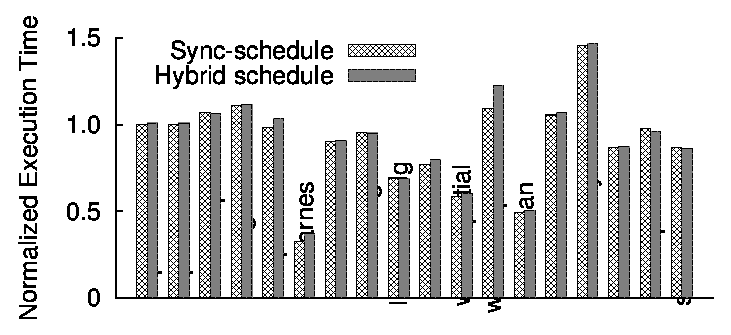
\includegraphics[width=\columnwidth]{peregrine/figures/overhead.eps}
\vspace{-.3in}
\caption{{\em Normalized execution time when reusing sync-schedules
    v.s. hybrid schedules.}  A time value greater than 1
  indicates a slowdown compared to a nondeterministic execution without
  \peregrine.  We did not include \racey because it was not designed for
  performance benchmarking. } \label{fig:overhead}
\end{figure}

For comparison, Figure~\ref{fig:overhead} shows the normalized
execution time when enforcing just the sync-schedules.  This overhead is
comparable to our previous work~\cite{cui:tern:osdi10}.  For all
programs except \watern, the overhead of enforcing hybrid schedules is only slightly
larger (at most 5.4\%) than that of enforcing sync-schedules.
This slight increase comes from two sources: (1) \peregrine has to enforce
execution order constraints to resolve races deterministically for \pbzip,
 \barnes, \fft, and \lun; and (2) the instrumentation framework \peregrine uses
also incurs overhead (\S\ref{sec:enforce-schedule}). 
The overhead for \watern increases by 13.4\% because it calls functions
more frequently than the other benchmarks, and our instrumentation framework
inserts code at each function entry and return
(\S\ref{sec:enforce-schedule}).


% We believe this slight overhead is well justified because hybrid
% schedules are fully deterministic whereas sync-schedules are not.

%% For XXX and XXX, \peregrine does not enforce
%% any execution order constraints, so the slowdown (average XXX\%) compared
%% to enforcing only sync-schedules comes solely from the instrumentation
%% framework.  For XXX and XXX, the slowdown (average XXX\%) compared to
%% enforcing only sync-schedules comes from both the instrumentation
%% framework and the execution order constraints.

\begin{figure}[b!]
\centering
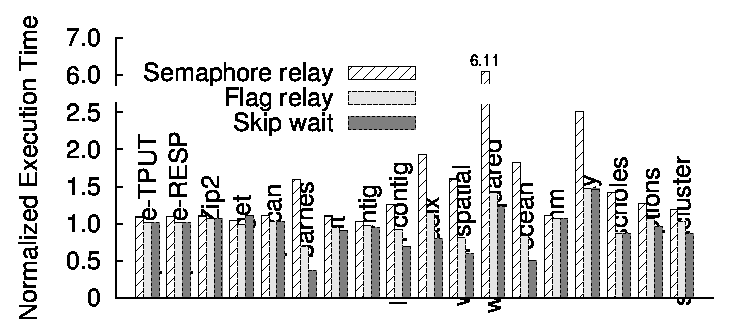
\includegraphics[width=\columnwidth]{peregrine/figures/opt.eps}
\vspace{-.3in}
\caption{{\em Speedup of optimization techniques.} Note that Y axis is
  broken.} \label{fig:opt}
\end{figure}

Figure~\ref{fig:opt} shows the speedup of flag relay
(\S\ref{sec:enforce-schedule}) and skipping blocking operations
(\S\ref{sec:nowait}).  Besides \watern and \cholesky, a
second group of programs, including \barnes, \lun, \radix, \waters, and
\ocean, also perform many synchronization operations, so flag relay speeds up
both groups of programs significantly.  Moreover, among the
synchronization operations done by the second group of programs, many are
\v{pthread\_barrier\_wait()} operations, so \peregrine further speeds up these
programs by skipping these wait operations.

%% For programs that do synchronization
%% operations frequently, such as \barnes, \lu, \watern, and \ocean, the
%% speedup can be huge.

%% For seven out of the
%% fourteen programs, the replayer performed almost identically to
%% nondeterministic execution. For \pbzip and barnes, \ds\ performed better.
%% This speedup came partially from the optimization to remove unnecessary
%% synchronizations, discussed in the next paragraph.  \ds's overhead for
%% MySQL, volrend, raytrace, water-nsquared, and choleskey is relatively
%% large because these programs performed many synchronization operations
%% over a short period of time.  For instance, water-nsquared and cholesky
%% both call \v{pthread\_mutex\_lock()} and \v{pthread\_mutex\_unlock()} in a
%% tight loop.

%% To better understand the replayer overhead, we analyzed the number of
%% execution order constraints it included in the schedule.
%% Table~\ref{tab:racy-edges} shows the results.  When recording execution
%% traces for these programs, \peregrine detected races for four programs: \pbzip,
%% FFT, LU, and BARNES.  It thus installs execution order constraints to
%% deterministically resolve the races.  Recall that to enforce execution
%% order constraints, \peregrine has to count branches for the racy regions of an
%% execution.  This branch counting incurs significant overhead.  In
%% addition, the more events in a schedule, the more conditionals \peregrine has to
%% include in the preconditions of the schedule.  Checking these
%% preconditions may incur significant overhead, too.  These factors are the
%% main factors that make LU and BARNES slower than DMT systems that enforce
%% sync-schedules.


%% \begin{table}[t]
%% \centering
%% \footnotesize
%% \begin{tabular}{lcccc}
%% {\bf Program} &  {\bf Nondet} &  {\bf Memoization} &  {\bf Overhead (times)}\\
%% \hline
%% \apache-TPUT   & 462.2 req/s         & 2.1 req/s                &   219.1\\
%% \apache-RESP   & 0.22 s        & 3.96 s            &   17.0\\
%% MySQL-TPUT    & 13779.3 req/s      & 172.2 req/s             &   79.0\\
%% MySQL-RESP    & 0.6 ms       & 61 ms             &   100.6\\
%% \pbzip        & 0.18 s        & 15.19 s           &   83.4\\
%% \end{tabular}
%% \caption{\small{\em Record overhead.}}
%% \label{tab:recorder-overhead}
%% \end{table}

%% {\bf Program} &{\bf Orig.}& {\bf Sync}  
%% \hline                               
%% \apache       &  672*     & 158         
%% \pbzip        &  280      & 304         
%% \aget         &  735      & 18788       
%% \pfscan       &   21      & 12308       
%% \barnes       &   21      & 12308       
%% \fft          &    9      & 101         
%% \lu           &    4      & 276         
%% \radix        &    2      & 348         
%% \waters       &    2      & 258         
%% \watern       &    2      & 1214        
%% \volrend      &   17      & 9781        
%% \ocean        &   32      & 12335       
%% \fmm          &    3      & 3098        
%% \cholesky     &   16      & 3882        
%% \blackscholes &   30      & 45          
%% \swaptions    &    1      & 47          
%% \streamcluster&    1      & 59          

\begin{table}[t]
\scriptsize
\centering
\begin{tabular}{crrrrrrr}
{\bf Program} &{\bf Trace}&{\bf Det} & {\bf Sli}  & {\bf Sim} & {\bf Sym} \\
\hline                                                                   
\apache       & 449       & 0.4      & 885.32     & n/a       & 5.8       \\
\pbzip        & 2,227     & 0.1      & 587.9      & 317.8     & 19.7      \\
\aget         & 233       & 0.4      & 78.8       & 60.1      & 13.2      \\
\pfscan       & 46,602    & 1.1      & 1,601.4    & 2,047.9   & 1,136.6   \\
\barnes       & 324       & 0.2      & 300.5      & 481.5     & 56.9      \\
\fft          & 39        & 0.0      & 2.1        & 3,661.7   & 0.4       \\
\luc          & 44,799    & 19.9     & 1,271.5    & 124.9     & 1,126.7   \\
\lun          & 41,302    & 21.2     & 1,999.8    & 14,243.8  & 1,201.0   \\
\radix        & 3,110     & 1.5      & 46.2       & 96.4      & 182.9     \\
\waters       & 7,508     & 1.0      & 1,407.0    & 9,628.1   & 120.6     \\
\watern       & 12,381    & 1.7      & 962.3      & 1,841.4   & 215.7     \\
\ocean        & 55,247    & 26.4     & 2,259.3    & 5,902.8   & 2,062.1   \\
\fmm          & 13,772    & 8.3      & 260.5      & 1,107.5   & 151.3     \\
\cholesky     & 47,200    & 28.8     & 3,102.9    & 6,350.1   & 685.5     \\
\blackscholes & 62,024    & 16.5     & 539.9      & 542.9     & 3,284.8   \\
\swaptions    & 1,366     & 0.0      & 23.2       & 87.3      & 1.2       \\
\streamcluster& 259       & 0.1      & 1.4        & 1.9       & 4.9       \\ 
\end{tabular}
\caption{{\em Analysis time.} {\bf Trace} shows the number of thousand
  LLVM instructions in the execution trace of the evaluated programs,
  the main factor affecting the execution time of \peregrine's various analysis
  techniques, including race detection ({\bf Det}), slicing ({\bf Sli}),
  simplification and alias analysis ({\bf Sim}), and symbolic execution
  ({\bf Sym}).  The execution time is measured in seconds.  The \apache
  trace is collected from one window of eight requests.  \apache uses
  thread pooling which our simplification technique currently does not
  handle well (\S\ref{sec:window}); nonetheless, slicing without simplification
  works reasonably well for \apache already
  (\S\ref{sec:stable}).} \label{tab:analysis-overhead}
\end{table}

%% \begin{table}[t]
%% \small
%% \centering
%% \begin{tabular}{cccc}
%% {\bf Program} & {\bf Nondet} & {\bf Recorder} & {\bf Overhead (times)}  \\
%% \hline
%% \apache-TPUT	& 672.45 (req/s) & 0.17 (req/s) & \\
%% \apache-RESP	& 0.001487s & 5765358 \\
%% pbzip		& 0.28s & 336063 & \\
%% AGET		& 0.735s & 13262446 & \\
%% pfscan		& 0.021s & 1136565938 & \\
%% barnes		& 0.0211s & 5686501 & \\
%% FFT		& 0.00873s & 414626 & \\
%% LU		& 0.00431s & 1201064595 & \\
%% RADIX		& 0.00236s & 182947144 & \\
%% WaterSpatial	& 0.00232s & 120580554 & \\
%% WaterNSquared	& 0.00228s & 215669938 & \\
%% volrend		& 0.0156s & 1668696976 & \\
%% ocean		& 0.0315s & 2062178214 & \\
%% fmm		& 0.00326s & 151372141 & \\
%% cholesky	& 0.0161s & 685491356 & \\
%% blackscholes	& 0.0297s & 3284752167 & \\
%% swaptions	& 0.00124s & 1277529 & \\
%% streamcluster	& 0.00131s & 4888817 & \\
%% \hline
%% \end{tabular}
%% \caption{{\em Recorder overhead.}} \label{tab:recorder-overhead}
%% \end{table}

%% \begin{table}[t]
%% \scriptsize
%% \centering
%% \begin{tabular}{cccccccc}
%% {\bf Program} & {\bf Trace} & {\bf Rec/Sym} & {\bf Race} & {\bf Slicing} & {\bf Simpl} & {\bf Sync}  \\
%% \hline
%% \apache & 449068 & 5765358 & 357341  & 885.32  & n/a  & 158  \\
%% \pbzip & 2227325 & 19722181 & 123413  & 587.88  & 317.76 & 304  \\
%% \aget & 233016 & 13262446 & 413488  & 78.76  & 60.12 & 18788  \\
%% \pfscan & 46601710 & 1136565938 & 1089680  & 1601.43  & 2047.92  & 12308   \\
%% \barnes & 323956 & 5686501 & 155723  & 300.50  & 481.45 & 12308  \\
%% \fft & 39340 & 414626 & 612  & 2.07  & 3661.72 & 101  \\
%% \lu & 41301696 & 1201064595 & 21209330  & 1999.77   & 14243.78 & 276  \\
%% \radix & 3109957 & 182947144 & 1528709  & 46.19   & 96.39 & 348  \\
%% \waters & 7508170 & 120580554 & 1004957  & 1407.04   & 9628.12  & 258  \\
%% \watern & 12380708 & 215669938 & 1650171  & 962.25   & 1841.35  & 1214  \\
%% \volrend & 112839700 & 1668696976 & 1160399  & tbd  & tbd & 9781  \\
%% \ocean & 55247263 & 2062178214 & 26429275  & 2259.33  & 5902.81  & 12335  \\
%% \fmm & 13771955 & 151372141 & 8252146  & 260.47  & 1107.49  & 3098  \\
%% \cholesky & 47200000 & 685491356 & 28757915  & 3102.94  & 6350.07 & 3882  \\
%% \blackscholes & 62024225 & 3284752167 & 16502100  & 539.87  & 542.88 & 45  \\
%% \swaptions & 1366447 & 1277529 & 41527  & 23.15  & 87.33 & 47  \\
%% \streamcluster & 259362 & 4888817 & 123222  & 1.35  & 1.91 & 59  \\
%% \end{tabular}
%% \caption{{\em Analysis time.} {\bf Trace} shows the number of LLVM IR
%%   instructions in the execution trace of each programs, the main factor
%%   that affects the execution time of \peregrine's various analysis techniques.
%%   Analysis time is measured in seconds.} \label{tab:analysis-overhead}
%% \end{table}

\para{Analyzer and recorder overhead.}  Table~\ref{tab:analysis-overhead}
shows the execution time of \peregrine's various program analyses.  The
execution time largely depends on the size of the execution trace.  All
analyses typically finish within a few hours.  For \pbzip and \fft, we
used small workloads (compressing 1~KB file and transforming a 256X256
matrix) to reduce analysis time and to illustrate that the schedules
learned from small workloads can be efficiently reused on large workloads.
The simplification and alias analysis time of \fft is large compared to its
slicing time because it performs many multiplications on array indexes,
slowing down our range analysis.  Although \lun and \luc implement the
same scientific algorithm, their data access patterns are very different
(\S\ref{sec:stable}), causing \peregrine to spend more time analyzing \lun than \luc.

\begin{figure}[b!]
\centering
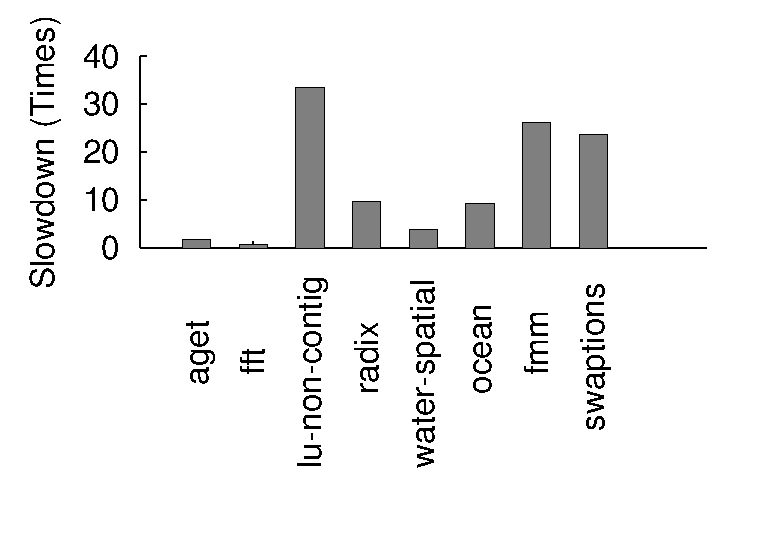
\includegraphics[width=.7\columnwidth]{peregrine/figures/new-recorder.eps}
\vspace{-.25in}
\caption{{\em Overhead of recording \v{load} and \v{store} instructions.}} \label{fig:new-recorder-overhead}
\end{figure}

As discussed in \S\ref{sec:record}, \peregrine currently runs \klee to record
executions.  Column Sym is also the overhead of \peregrine's recorder.  This
crude, unoptimized recorder can incur large slowdown compared to
the normal execution of a program.  However, this slowdown can be reduced
to around 10X using existing record-replay
techniques~\cite{idna:vee06,scribe:sigmetrics10}.  Indeed, we have
experimented with a preliminary version of a new recorder that records an
execution by instrumenting \v{load} and \v{store} instructions and saving
them into per-thread logs~\cite{idna:vee06}.  Figure~\ref{fig:new-recorder-overhead} shows that
this new recorder incurs roughly 2-35X slowdown on eight programs,
comparable to existing record-replay systems.  Due to time
constraints, we have not integrated this new recorder with \peregrine.

%% this large slowdown is mainly
%% due to our crude implementation.  The interpretation alone adds roughly
%% 10x overhead.

%% Fortunately, the functionality of our recorder is very similar to other
%% systems that deterministically record executions.  Thus, existing
%% techniques~\cite{idna:vee06,scribe:sigmetrics10} may directly speed up our
%% recorder.  Indeed, we have implemented a preliminary version of an LLVM IR
%% recorder that records an execution by instrumenting load/store
%% instructions and recording them into per-thread logs, borrowing ideas from
%% previous work~\cite{idna:vee06}.  Table~\ref{tab:new-recorder-overhead}
%% shows the overhead of this new recorder on XXX programs, which is around
%% 10 times.  Due to time constraints, we have not integrated it with \peregrine.

\subsection{Stability} \label{sec:stable}

Stability measures how frequently \peregrine can reuse schedules.  The more
frequently \peregrine reuses schedules, the more efficient it is, and the
more repeatable a program running on top of \peregrine becomes.  While \peregrine
achieves determinism and efficiency through hybrid schedules, it may have
to pay the cost of slightly reduced reuse rates compared to a
manual approach~\cite{cui:tern:osdi10}.

%  because the preconditions it computes are not always the weakest
%  preconditions (\S\ref{sec:slice}).

% That is, \peregrine's slicing technique may have to include conditionals that
% affect neither determinism or feasibility of a schedule, thus reducing
% schedule-reuse rates.

%% \begin{figure}[t]
%% \centering
%% \includegraphics[width=0.4\textwidth]{figures/slicing}
%% \caption{{\em Slicing ratio.}  The smaller the ratio, the
%%   more effective our slicing technique is.} \label{fig:slice-ratio}
%% \end{figure}

%% \begin{table}[t]
%% \small
%% \centering
%% %\begin{tabular}{ccccc}
%% %\multirow{2}{*}{\bf Program} & \multirow{2}{*}{\bf UB} 
%% %& \multicolumn{2}{c}{\bf \peregrine}
%% %\multirow{2}{*}{\bf LB} 
%% %& & {\bf Slicing} & {\bf Simplification} & \\
%% \begin{tabular}{ccccc}                
%% \multirow{2}{*}{\bf Program} & \multirow{2}{*}{\bf UB}
%% & \multicolumn{2}{c}{\bf \peregrine}             
%% & \multirow{2}{*}{\bf LB} \\
%% & & {\bf Slicing} & {\bf Simplification} & \\  
%% \hline
%% \apache        & 449068 & 88956 & n/a \\
%% \pbzip         & 2227325 & 1398208 & 1584 \\
%% \aget          & 233016 & 141417 & 103833 \\
%% \pfscan        & 46601710 & 29943748 & 24745296 \\
%% \barnes        & 323956 & 133340 & 127272 \\
%% \fft           & 39340 & 20284 & 2230 \\
%% \lu            & 41301696 & 31726764 & 31629294 \\
%% \radix         & 3109957 & 1129498  & 865133 \\
%% \waters        & 7508170 & 2997156 & 1782261 \\
%% \watern        & 12380708 & 6072770 & 1878349 \\
%% \volrend       & tbd & tbd & tbd \\
%% \ocean         & 55247263 & 29336752 & 28714504 \\
%% \fmm           & 13771955 & 1728660 & 1705497 \\
%% \cholesky      & 47200000 & 12239760 & 11059092 \\
%% \blackscholes  & 62024225 & 3317961 & 197 \\
%% \swaptions     & 1366447 & 803884 & 180 \\
%% \streamcluster & 259362 & 875 & 222 \\
%% \end{tabular}
%% \caption{{\em Number of instructions.}  {\bf UB}
%%   shows the total number of instructions in the corresponding execution
%%   trace.  {\bf Slicing} and {\bf Simplification} show the number of
%%   instructions in the trace slice after applying determinism-preserving
%%   slicing (\S\ref{sec:slice}) alone and after further applying
%%   schedule-guided simplification
%%   (\S\ref{sec:guide}). } \label{tab:slice-inst-ratio}
%% \end{table}


\begin{figure}[t]
\centering
\includegraphics[width=\columnwidth]{peregrine/figures/slicing.eps}
\vspace{-.3in}
\caption{{\em Slicing ratio after applying determinism-preserving slicing alone 
    (\S\ref{sec:slice}) and after further applying schedule-guided
    simplification (\S\ref{sec:guide}).}} \label{fig:slice-ratio}
\vspace{-.05in}
\end{figure}

A key factor determining \peregrine's schedule-reuse rates is how effectively it
can slice out irrelevant instructions from the execution traces.
Figure~\ref{fig:slice-ratio} shows the ratio of the slice size over the trace size for
\peregrine's determinism-preserving slicing technique, with and without
schedule-guided simplification.  The slicing technique alone reduces the
trace size by over 50\% for all programs except \pbzip, \aget, \pfscan,
\fft, \lun, \ocean, and \swaptions.  The slicing technique combined with
scheduled-guide simplification vastly reduces the trace size for \pbzip,
\aget, \fft, \luc, and \swaptions.

Recall that \peregrine computes the preconditions of a schedule from
the input-dependent branches in a trace slice.  The
fewer branches included in the slice, the more general the preconditions
\peregrine computes tend to be.  We further measured the number of such
branches in the trace slices.  Table~\ref{tab:slice-ratio} shows the
results, together with a upper bound determined by the total number of
input-dependent branches in the execution trace, and a lower bound
determined by only including branches required to reach the recorded
synchronization operations.  This lower bound may not be tight as we ignored data
dependency.  For \barnes, \fft, \blackscholes, \swaptions, and
\streamcluster, slicing with simplification (Column ``Slicing+Sim'')
achieves the best possible reduction.  For \pbzip, \aget, \pfscan, and \luc, the
number of input-dependent branches in the trace slice is close to the
lower bound.  In the remaining programs, \apache, \fmm, and \cholesky
also enjoy large reduction, while the other five programs do not.  This table
also shows that schedule-guided simplification is key to reduce the
number of input-dependent branches for \pbzip, \fft, \luc, \blackscholes, 
and \swaptions,
and to reach the lower bound for \blackscholes, \swaptions, and \streamcluster.

%% \peregrine's program analysis techniques combined ({\bf Simplification} column)
%% effectively remove a large number of input-dependent conditionals, vastly
%% increasing schedule reuse rates.  It achieves the best possible reduction
%% for \blackscholes, \swaptions, and \fft.

%% We evaluated \peregrine's stability with two experiments.  First, we quantified
%% the number of input-dependent conditionals after each program
%% analysis technique was applied.  

%% Table~\ref{tab:slice-ratio} also shows the effects of each program
%% analysis technique in \peregrine.  Determinism-preserving slicing greatly
%% reduces the number of input-dependent conditionals for \pbzip, \aget, and
%% \swaptions.  Schedule-guided simplification helps further reduce this
%% number further for \aget, \fft, and \blackscholes.  Both techniques are
%% useful.

%% First, we measured
%% \apache's stability with \peregrine over a real HTTP trace with 122,000 HTTP
%% requests.  We first randomly selected 1\% of the workload, and used the
%% workload to populate a schedule cache.  We then replayed the entire trace
%% at a rate of 100 concurrent requests/s to \apache on top of \peregrine.  We
%% measured a cache hit rate of 82.3\%, slightly lower than previous
%% work~\cite{cui:tern:osdi10}.

%% To quantify the effectiveness of \peregrine's slicing technique, we measured the
%% ratio of an trace slice over an execution trace.
%% Figure~\ref{fig:slice-ratio} shows the results.  For FFT, LU, and RADIX,
%% \peregrine effectively computed a path slice smaller than 10\% of the execution
%% trace.  For \apache, PBZip2, and BARNES, this ratio is higher, but still
%% less than 30\%.

We manually examined the preconditions \peregrine computed from the
input-dependent branches for these programs.  We category these programs
below.

%\begin{tightenum}
%\item[$\bullet$] 
\para{Best case}: \pbzip, \fft, \luc, \blackscholes, \swaptions,
  and \streamcluster. \peregrine computes the weakest (\ie, most relaxed) preconditions
  for these programs.  The preconditions often allow \peregrine to reuse
  one or two schedules for each number of threads, putting no
   or few constraints on the data processed.
  Schedule-guided simplification is crucial for
  these programs; without simplification, the preconditions
  would fix the data size and contents.

\para{Slicing limitation}: \apache and \aget. The
  preconditions \peregrine computes for \apache fix the URL length; they also
  constrain the page size to be within an 8~KB-aligned range if
    the page is not cached.  The preconditions \peregrine computes for \aget fix
    the positions of ``\v{/}'' in the URL and narrow down the file size
    to be within an 8~KB-aligned range.  These preconditions thus
      unnecessarily reduce the schedule-reuse rates.  Nonetheless, they
      can still match many different inputs, because they do not constrain
      the page or file contents.

\para{Symbolic execution limitation}: \barnes.  \barnes
  reads in two floating point numbers from a file, and their values affect
  schedules.  Since \peregrine cannot symbolically execute floating point
  instructions, it currently does not collect preconditions from them.
  % these instructions.
%%   conservatively adds preconditions to fix the
%%   values of these numbers.  Even so, \peregrine can still reuse the schedules
%%   regardless of the other data sizes and contents.

\para{Alias limitation}: \lun, \radix, \waters, \watern, \ocean,
  and \cholesky.  Even with simplification, \peregrine's alias analysis
  sometimes reports may-alias for pointers accessed in different threads,
  causing \peregrine to include more instructions than necessary in the
  slices and compute preconditions that fix the input data.  For
  instance, each thread in \lun accesses disjoint regions in a global
  array, but the accesses from one thread are \emph{not} continuous,
  confusing \peregrine's alias analysis.  (In contrast, each thread in \luc accesses
  a contiguous array partition.)
% gets confused and considers accesses from   different threads as aliases.

\para{Programs that rarely reuse schedules}: \pfscan and
  \fmm.  For instance, \pfscan searches a keyword in a set of files using
  multiple threads, and for each match, it grabs a lock to increment a
  counter.  A schedule computed on one set of files is unlikely to suit
  another.

\begin{table}[t]
\small
\centering
\begin{tabular}{crrrr}
\multirow{2}{*}{\bf Program} & \multirow{2}{*}{\bf UB} 
& \multicolumn{2}{c}{\bf \peregrine} 
& \multirow{2}{*}{\bf LB} \\
& & {\bf Slicing} & {\bf Slicing+Sim} & \\
\hline
\apache       &  4,522   &  624    & n/a      & 56     \\
\pbzip        &  913     &  865    & 101      & 94     \\
\aget         & 20,826   & 18,859  & 9,514    & 9,491  \\
\pfscan       & 1,062,047& 992,524 & 992,520  & 992,501\\
\barnes       &  92      & 52      & 52       & 52     \\
% This is fft -p8 -m6 slicing results, not m16. Range analysis currently can not run m16.
\fft          &  2,266   & 1,568   & 17       & 17     \\
\luc          &2,823,379 &2,337,431& 131      & 128    \\
\lun          &2,962,621 &2,877,877& 2,876,364& 128    \\
\radix        &  175,679 & 98,750  & 89,732   & 75     \\
\waters       &  98,054  & 77,567  & 76,763   & 233    \\
\watern       &  89,348  & 76,786  & 76,242   & 1,843  \\
\ocean        &2,605,185 &2,364,538&2,361,256 & 400    \\
\fmm          &  299,816 & 57,670  & 56,532   & 1,642  \\
\cholesky     &  7,459   & 1,627   & 1,627    & 1,233   \\
\blackscholes & 421,909  & 409,618 & 10       & 10 \\
\swaptions    & 35,584   & 35,005  & 21       & 21 \\
\streamcluster& 20,851   & 75      & 42       & 42 \\
\end{tabular}
\vspace{-.1in}
\caption{{\em Effectiveness of program analysis techniques.}  {\bf UB}
  shows the total number of input-dependent branches in the
  corresponding execution trace, an upper bound on the number included in 
  the trace slice.  {\bf Slicing} and {\bf Slicing+Sim} show the
  number of input-dependent branches in the slice after applying
  determinism-preserving slicing alone (\S\ref{sec:slice}) and after
  further applying schedule-guided simplification
  (\S\ref{sec:guide}). {\bf LB} shows a lower bound on the number of
  input-dependent branches, determined by only including branches
  required to reach the recorded synchronization operations.
  This lower bound may not be tight as we ignored data
  dependency when computing it.} \label{tab:slice-ratio}
\vspace{-.05in}
\end{table}



%% compared the preconditions \peregrine computed for \splash
%% benchmarks to the preconditions computed based on our manual
%% annotations~\cite{cui:tern:osdi10}.  For \fft, the preconditions \peregrine
%% computed match our previous results: as long as the number of threads
%% remains the same, we can reuse a schedule on an input, regardless of other
%% command line arguments.  For XXX, the preconditions \peregrine automatically
%% inferred are indeed more stringent than then manual annotations given
%% in~\cite{cui:tern:osdi10}.  TODO.  Nonetheless, \peregrine sliced out all other
%% command line arguments, thus still allowing frequent reuses of schedules.

% file contains \pbzip headers

%% reuse less frequently than previous system.

%%   - pbzip2: reuse rate

%%   - apache: reuse rate

%%   - manual comparison of splash2 benchmarks

%%     best constraints v.s. constraints extracted

% \subsection{Effectiveness of Program Analysis Techniques} \label{sec:opt}

%% % determinism-preserving slicing

%% % scheduled-guided analysis

%%   number of branch instructions in the execution trace 

%%   number of branch instructions in the trace slice (after slicing, without
%%   max slicing )

%%   number of branch instructions in the trace slice (after slicing, with
%%   max slicing )

%%   number of may-race (races due to may-alias), including

%% \begin{tightenum}
%% \item    instruction, instruction

%% \item    branch, instruction

%% \item    branch, brandh
%% \end{tightenum}


\subsection{Ease of Use} \label{sec:annotation}

\begin{table}[t]
\centering
\small
\begin{tabular}{crcc}
{\bf Program} & {\bf LOC} & {\bf \peregrine} & {\bf \tern} \\
\hline
% -6.0 
\apache       & 464~K   & 24  & 6  \\
\pbzip        & 7,371  & 1   & 3  \\
\aget         &   834  & 0   & n/a\\
\pfscan       &   776  & 0   & n/a\\
\barnes       & 1,954  & 0   & 9  \\
\fft          & 1,403  & 1   & 4  \\   
\luc          & 991    & 0   & n/a  \\ 
\lun          & 1,265  & 0   & 3  \\   
\radix        & 661    & 0   & 4  \\   
\waters       & 1,573  & 0   & 9  \\
\watern       & 1,188  & 0   & 10 \\
\ocean        & 6,494  & 0   & 5  \\
\fmm          & 3,208  & 0   & 9  \\
\cholesky     & 3,683  & 0   & 4  \\
\blackscholes & 1,275  & 0   & n/a\\
\swaptions    & 1,110  & 0   & n/a\\
\streamcluster& 1,963  & 0   & n/a\\
\racey        & 124    & 0   & n/a\\
\end{tabular}
\vspace{-.05in}
\caption{{\em Source annotation requirements of \peregrine v.s. \tern.}  {\bf
    \peregrine} represents the number of annotations added for \peregrine, and {\bf
    \tern} counts annotations added for \tern.  Programs not included in
  the \tern evaluation are labeled n/a. LOC of \pbzip also includes the
  lines of code of the compression library \v{libbz2}.} \label{table:apps}
\vspace{-.05in}
\end{table}

Table~\ref{table:apps} shows the annotations (\S\ref{sec:func-summary}) we
added to make the evaluated programs work with \peregrine.  For most programs,
\peregrine works out of the box.  \apache uses its own library functions for
common tasks such as memory allocation, so we annotated 21 such
functions.  We added two annotations to mark the boundaries of client
request processing and one to expose the hidden state
in \apache (\S\ref{sec:window}).  \pbzip decompression
uses a custom search function (\v{memstr}) to scan through the input file
for block boundaries.  We added one annotation for this function to relax
the preconditions \peregrine computes.  (\peregrine works automatically with \pbzip
compression.)  We added one assertion to annotate the range of a variable
in \fft (\S\ref{sec:func-summary}).

For comparison, Table~\ref{table:apps} also shows the annotation overhead of our previous DMT system \tern~\cite{cui:tern:osdi10}.  For all programs except \apache, \peregrine
has fewer number of annotations than \tern.  Although the number
of annotations that \tern has is also small, adding these annotations may
require developers to manually reconstruct the control- and
data-dependencies between instructions.
% within a thread as well as across threads.

% emphasize interesting side effects
In order to make the evaluated programs work with \peregrine, we had to fix several bugs
in them.  For \aget, we fixed an off-by-one write in \v{revstr()} which
prevented us from tracking constraints for the problematic write, and a
missing check on the return value of \v{pwrite()} which prevented us from
computing precise ranges.  We fixed similar missing checks in \swaptions,
\streamcluster, and \radix.  We did not count these modifications in
Table~\ref{table:apps} because they are real bug fixes.  (This interesting
side-effect illustrates the potential of \peregrine as an error detection tool:
the precision gained from simplification enables \peregrine to detect real races
in well-studied programs.)

% fft: inlined three functions


\section{Related Work} \label{sec:related}

\noindent
{\bf Deterministic Execution} \tern differs from existing \dmt
systems~\cite{dmp:asplos09,coredet:asplos10,kendo:asplos09} by making
threads stable, \ie, repeating familiar behaviors across different inputs.
Another difference is that \tern reduces timing nondeterminism for server
programs through windowing.

% \tern is a software-only approach for multithreaded programs with general
% semantics (\eg, not fork-join~\cite{grace:oopsla09}) and written in legacy
% languages such as C and C++, in contrast to new programming languages
% (\eg~\cite{shim,streamit}), hardware-based approaches~\cite{dmp:asplos09}, and
% systems for programs with restricted semantics~\cite{grace:oopsla09}.

The closest system to \tern in this category is
Kendo~\cite{kendo:asplos09}, a software-only \dmt system that also
enforces synchronization orders instead of memory access orders for
efficiency.  \coredet~\cite{coredet:asplos10} is another software-only \dmt
system that enforces deterministic memory access orders.  Both systems are
based on logical clocks and have been shown to work on scientific
benchmarks, such as \splash.  The authors of \coredet have noted that a small
modification to the original program leads to a much different
\coredet-instrumented program, which the idea of schedule memoization may
address.  \coredet is a software implementation (with extensions) of
DMP~\cite{dmp:asplos09}, a hardware \dmt system .

Grace~\cite{grace:oopsla09} proposes a novel approach to making C and C++
programs with fork-join parallelism behave like sequential programs.  It
runs each thread within a process and commits memory writes atomically and
deterministically.  It detects memory access conflicts efficiently using
hardware page protection.  Grace has been shown to perform and scale well
on Phoenix benchmarks~\cite{phoenix-benchmarks} and a Cilk~\cite{cilk}
benchmark.  Unlike Grace, \tern aims to make general multithreaded
programs, not just fork-join programs, deterministic and stable.

%Several new program languages can make programs
%written in them deterministic.  Although a language-based approach may be
%the ultimate solution to determinism and stability, existing 

\noindent
{\bf Deterministic Replay} Deterministic
replay~\cite{r2:osdi,friday2007,srinivasan:flashback,revirt,dejavu,vmware-record-replay,smp-revirt:vee08,pres:sosp09,scribe:sigmetrics10,odr:sosp09,capo:asplos09}
aims to replay the exact recorded executions, whereas \tern ``replays''
memoized schedules on different inputs.  Some recent deterministic replay
systems include Scribe, which tracks page ownership to enforce
deterministic memory access~\cite{scribe:sigmetrics10}; Capo, which defines
a novel software-hardware interface and a set of abstractions for
efficient replay~\cite{capo:asplos09}; PRES and ODR, which
systematically search for a complete execution based on a partial
one~\cite{pres:sosp09,odr:sosp09}; and SMP-ReVirt, which uses clever page
protection trick for recording the order of conflicting memory
accesses~\cite{smp-revirt:vee08}.

\noindent
{\bf Concurrency Errors} The complexity in developing multithreaded
programs has led to many concurrency errors~\cite{lu:concurrency-bugs}.  A
significant number of them are not data races, but atomicity and order
errors~\cite{lu:concurrency-bugs}, which can be deterministically
reproduced or avoided using only synchronization orders.

Much work exists on concurrency error
detection~\cite{yu:racetrack:sosp,savage:eraser,racerx:sosp03,lu:muvi:sosp,avio:asplos06,conmem:asplos10},
diagnosis~\cite{racefuzzer:pldi08,ctrigger:asplos09,atomfuzzer:fse08}, and
correction~\cite{dimmunix:osdi08,gadara:osdi08}.  \tern aims to make the
executions of multithreaded programs deterministic and stable, and is
complementary to existing work on concurrency errors.  Specifically,
\tern can use existing work to detect and fix the errors in the schedules
it selects.  Moreover, even for programs free of concurrency errors,
\tern still provides value by making their behaviors repeatable.

\noindent {\bf Symbolic Execution} The combination of symbolic and
concrete executions has been a hot research topic.  Researchers have built
scalable and effective symbolic execution systems to detect
errors~\cite{dart:pldi,cute:fse,godefroid:grammar-fuzzing,godefroid:whitebox-fuzzing,klee:osdi08,yang:malicious-disk:oakland06,cadar:exe:ccs06,s2e:hotdep09,taas:socc10},
block malicious inputs~\cite{castro:bouncer}, and preserve privacy in
error reports~\cite{castro:bug-report-privacy}.  Compared to these
systems, \tern applies symbolic execution to a new domain: tracking input
constraints to reuse schedules.

\chapter{Conclusion} \label{sec:conclusion}

Multithreading is notoriously difficult to get right, and our research reveals
that a key reason is: a multithreaded program may run into exponentially many
possible schedules for all inputs at runtime, which brings a series of
significant reliability and security challenges on understanding,
testing, debugging, analyzing, verification, and replication of multithreaded
programs.

To reduce the number of possible schedules and make multithreaded
programs easier to get right, we have invented a new idea called Stable
Multithreading (or \smt) that reuses each schedule on a wide range of inputs,
greatly reducing the number of possible schedules for all inputs. Through
building three \smt systems, \tern, \peregrine, and \parrot, with each addressing
a distinct research challenge, we have shown that \smt can be made simple, fast,
and deployable. Through applying \smt to make reproducing concurrency bugs
easier, to improve precision of static program analysis, and to increase
coverage of model checking tools, we have quantitatively shown that \smt can
make multithreaded programs much easier to get right. All the source code,
benchmarks, and raw evaluation results of our latest \smt system \parrot are
available at: \github. In addition to our effort on building and applying \smt
systems, some techniques and ideas in our \tern and \peregrine systems have been
leveraged by University of Washington researchers to compute a small set of
schedules to cover all or most inputs of multithreaded programs.

By addressing the key reason that makes multithreading difficult to get right,
\smt has broad applications. In the future, we plan to apply \smt to make
replication and verification of multithreaded programs easier, and to defend
against security vulnerabilities that leverage concurrency bugs. We believe that
all these combined effort will make \smt a simple, fast, reliable, and secure
multithreading runtime, potentially benefiting all individuals, governments,
organizations, and software vendors. 
~\\[1in] % hack to put space at top.
\textbf{\Huge Acknowledgments}\\

\noindent 
I extend special thanks to my advisor, Prof. Junfeng Yang, who has supported and directed all aspects of my PhD career. I also sincerely thank Prof. Jason Nieh, Prof. Gail Kaiser, Prof. Roxana Geambasu, Prof. Jinyang Li, Prof. Randal E. Bryant, Prof. Garth A. Gibson, Prof. Simha Sethumadhavan, and Prof. Martha Kim for their valuable suggestions, advice, and collaboration during my PhD study. Parts of this thesis were joint work with Dr. Jingyue Wu, Dr. Jiri Simsa, Chia-che Tsai, John Gallagher, Huayang Guo, Yang Tang, Gang Hu, Yi-Hong Lin, Dr. Hao Li,  Ben Blum, and Xinan Xu. I also extend thanks to Jonathan Bell, Adrian Tang, and Yunfei Wang for their feedback and comments on my research.

\end{sloppypar}

% uncomment to tweak with bib spacing
%\setlength\bibsep{2.25pt}
{
%\small
 \bibliographystyle{abbrvnat}
 \bibliography{bib/biblio}
}

\end{document}
